\documentclass{article}
\usepackage[utf8]{inputenc}
\usepackage[spanish]{babel}
\usepackage{geometry}
 \geometry{
 a4paper,
 total={170mm,257mm},
 left=20mm,
 top=20mm,
 }
\usepackage{graphicx}
\usepackage{titling}
\usepackage[hidelinks=true]{hyperref}
\usepackage{amsmath}
\usepackage{amssymb}
\usepackage{amsthm}
\usepackage{mdframed}
\usepackage{xcolor}
\usepackage{verbatim}
\usepackage{marginnote}
\usepackage{background}
\usepackage[most]{tcolorbox}
\usepackage{tikz}
\usetikzlibrary{calc} 
\usepackage{varwidth}
\usepackage{pifont}

\backgroundsetup{
    scale=5,
    color=gray!40,          % Color gris claro
    opacity=0,
    angle=45,
    position=current page.center,
    contents={Sistemas Operativos - FaMAF 2024}
}

% --------- Colores ------------ %
\definecolor{coralred}{rgb}{1.0, 0.25, 0.25}
\definecolor{crimson}{rgb}{0.86, 0.08, 0.24}
\definecolor{pastelmagenta}{rgb}{0.96, 0.6, 0.76}
\definecolor{darkbyzantium}{rgb}{0.36, 0.22, 0.33}
\definecolor{whitesmoke}{rgb}{0.96, 0.96, 0.96}
\definecolor{cinnabar}{rgb}{0.89, 0.26, 0.2}

\tcbuselibrary{breakable}

\newtcolorbox{definition}{
 enhanced,breakable,
 before skip=0.8cm,after skip=0.8cm,
 bottom=0.5cm,colframe=crimson,coltitle=white,
 colback=coralred!4,boxrule=0.2mm,arc=0mm,leftrule=2mm,
 attach boxed title to top left={xshift=0cm,yshift*=0mm-\tcboxedtitleheight},
 varwidth boxed title*=-3cm,
 boxed title style={frame code={
   \coordinate (A) at (frame.north east);
   \coordinate (B) at (frame.south east);
   \path[fill=coralred](frame.north east)--([xshift=-2mm]frame.north west)--([xshift=-2mm]frame.south west)--(frame.south east) --([xshift=3mm]$(A)!0.5!(B)$)--cycle;
   \draw[white,line width=2pt]([xshift=-2mm]frame.north east)--([xshift=1mm]$(A)!0.5!(B)$)--([xshift=-2mm]frame.south east);
   \path[fill=coralred!50]([xshift=-2mm]frame.south west)--+(2mm,-2mm)|-cycle;
  },interior engine=empty,
 },
 title={\bf\color{white} \large Definición}
}

\newtcolorbox{solution}[1][]{
 colframe=pastelmagenta,
 colback=pastelmagenta!12!white,
 boxed title style={colback=pastelmagenta},
 breakable,
 enhanced,
 sharp corners,
 boxsep=1pt,
 attach boxed title to top left={yshift=-\tcboxedtitleheight,  yshifttext=-1.05\baselineskip},
 boxed title style={boxsep=1pt,sharp corners},
 fonttitle=\bfseries\sffamily,
 no shadow,
 top=1ex,
 boxrule=0pt,
 leftrule=1.4pt,
 title={\color{darkbyzantium} Solución \fontsize{14}{16.8}\ding{45}},
 colframe=pastelmagenta,
 colback=pastelmagenta!12!white,
 boxed title style={colback=pastelmagenta},
 overlay unbroken and first={
 \node[below right,font=\small,color=magenta,text width=.8\linewidth]
 at (title.north east) {#1};
}}

\newtcolorbox[auto counter, number within=section]{summary}[2][]{ % 2 argumentos: [opciones] y {título}
  breakable,
  top=1cm,
  title={#2}, % Usa el segundo argumento para el título
  enhanced,
  before skip=5mm,
  after skip=5mm,
  boxsep=3mm,
  colback=whitesmoke,
  coltitle=white,
  attach boxed title to top left={xshift=5mm,yshift=-\tcboxedtitleheight},
  boxrule=.5pt,
  boxed title style={
    interior empty,
    frame code={
      \fill([xshift=1mm]frame.north east)arc(180:0:1mm)([xshift=-1mm]frame.north west)arc(0:180:1mm);
      \path[right color=cinnabar,left color=cinnabar,middle color=cinnabar!80] ([shift={(-.2,.1)}]frame.north west)--([shift={(.2,.1)}]frame.north east)[rounded corners=1mm]--([xshift=.1cm]frame.north east)--(frame.south east)--(frame.south west)--([xshift=-.1cm]frame.north west)[sharp corners]--cycle;
    }
  }
}


%\definecolor{lightgray}{gray}{0.95} 
%\pagecolor{lightgray}              

 \title{Sistemas Operativos 2024 \\ Parte I - Virtualización - Notas Teóricas}
\author{Villar Pedro}
\date{\today}

\usepackage{fancyhdr}
\pagestyle{fancy}
\fancyhf{}
\lhead{Villar Pedro}
\rhead{UNC - FaMAF}

\lfoot{Sistemas Operativos 2024}
\rfoot{\thepage}



\makeatletter
\def\@maketitle{%
  \newpage
  \null
  \vskip 1em%
  \begin{center}%
  \let \footnote \thanks
    {\LARGE \@title \par}%
    \vskip 1em%
    %{\large \@date}%
  \end{center}%
  \par
  \vskip 1em}
\makeatother

\begin{document}

\maketitle

\noindent\begin{tabular}{@{}ll}
    Estudiante & \theauthor\\
    Profesor &  Nicolas Wolovick\\
\end{tabular}

\tableofcontents
\newpage
\listoffigures
\newpage
\section{Procesos}
Un programa es un objeto estático, mientras que un proceso es un objeto dinámico. Siempre que hablemos de procesos o programas vamos a estar hablando de código maquina. El SO toma este objeto estático, luego acomoda toda la memoria, luego carga este objeto estático en memoria y lo ejecuta, convirtiéndolo en un objeto dinámico, el proceso. 
\begin{definition}
    Un proceso es una instancia de un programa en ejecución, en cambio un programa es un archivo que contiene una variedad de información que describe como construir un proceso en tiempo de ejecución. Un programa puede usarse para construir muchos procesos o, dicho de otro modo, muchos procesos pueden estar ejecutando el mismo programa.

    Si hablamos en términos del kernel, un proceso es una entidad abstracta, definida por el kernel, a la cual se le asignan recursos del sistema para ejecutar un programa. Desde el punto de vista del kernel, un proceso consiste en memoria en el espacio de usuario que contiene el código del programa y las variables utilizadas por dicho código, así como una serie de estructuras de datos del kernel que mantienen información sobre el estado del proceso. La información registrada en estas estructuras de datos del kernel incluye varios números identificadores (IDs) asociados con el proceso, tablas de memoria virtual, la tabla de descriptores de archivos abiertos, información relacionada con la entrega y manejo de señales, uso y límites de recursos del proceso, el directorio de trabajo actual, y una multitud de otra información. 
    \footnote{The Linux programming interface}
\end{definition}

Con esto surge un \textbf{problema}, si se tienen dos cores y cuatro procesos, los cuales se quieren ejecutar en los cores. Se quiere saber si es posible ejecutar los procesos en los cores de manera tal que se maximice la utilización de los cores.

¿Cómo se resuelve este problema? Se realiza a través de \textbf{mecanismos de bajo nivel}, código de máquina con ciertas instrucciones especiales de la CPU, la CPU real se distribuye mediante lo llamado \textbf{políticas}. Es decir que las política son el cómo se van a distribuir esos recursos escasos entre los procesos. Las políticas de Planificación y los planificadores son los encargados de esto.

\footnote{OSTEP Cap.4: La Abstracción de los Procesos}

\subsection{Definición y rol del SO}
Podemos definir al proceso o tarea como la abstracción de un programa en ejecución. Un proceso es un conjunto que reune lo siguiente:
\begin{itemize}
    \item Las \textbf{instrucciones y datos} del programa, también conocido como \textit{espacio de direcciones}.
    \item Información sobre el \textbf{estado} de la ejecución del programa.
    \item Información de \textbf{control} sobre el programa para el SO.
\end{itemize}
El sistema operativo se va a encargar de lo siguiente:
\begin{itemize}
    \item Intercalar la ejecución de los procesos en un orden tal que maximiza la utilización del procesador.
    \item Gestionar y asignar los otros recursos del sistema (memoria, E/S, etc.) para que los procesos puedan hacer uso de ellos.
    \item Gestionar la comunicación de datos entre diferentes procesos presentes en el sistema.
    \item Ayudar en la creación de nuevos procesos por parte de los usuarios.
\end{itemize}

\footnote{Clase 3 - Hugo Carrer - FCEFyN - UNC}

\section{API de Procesos}
Las operaciones típicas que se pueden realizar sobre un proceso son \textbf{crear}, \textbf{liberar recursos}, \textbf{esperar}, \textbf{controlar} y \textbf{saber su estado}:
\begin{itemize}
    \item[$\looparrowright$] \textbf{Crear:} Un sistema operativo debe incluir algún método para crear nuevos procesos. Cuando escribes un comando en la shell o haces doble clic en el ícono de una aplicación, el sistema operativo es invocado para crear un nuevo proceso que ejecute el programa que has indicado.
    \item[$\looparrowright$] \textbf{Liberar recursos:} Así como hay una interfaz para la creación de procesos, los sistemas también proporcionan una interfaz para destruir procesos de manera forzada. Por supuesto, muchos procesos se ejecutarán y saldrán por sí mismos cuando terminen; sin embargo, cuando no lo hacen, el usuario puede desear matarlos, y por lo tanto, una interfaz para detener un proceso descontrolado es bastante útil.
    \item[$\looparrowright$] \textbf{Esperar:} A veces, un proceso necesita esperar a que otro proceso termine antes de continuar. Por ejemplo, un proceso puede necesitar esperar a que un proceso hijo termine antes de continuar. En este caso, el proceso padre puede esperar a que el proceso hijo termine.
    \item[$\looparrowright$] \textbf{Controlar:} Además de matar o esperar un proceso, a veces existen otros controles posibles. Por ejemplo, la mayoría de los sistemas operativos proporcionan algún tipo de método para suspender un proceso (detener su ejecución por un tiempo) y luego reanudarlo (continuar su ejecución).
    \item[$\looparrowright$] \textbf{Saber su estado:} Por lo general, hay interfaces para obtener información sobre el estado de un proceso, como cuánto tiempo ha estado ejecutándose o en qué estado se encuentra.
\end{itemize}
\subsection{Creación de procesos}
Tenemos que transformar un programa en un proceso, lo primero que debe hacer el sistema operativo para ejecutar un programa es cargar su código y cualquier dato estático en la memoria, dentro del espacio de direcciones del proceso. Inicialmente, los programas residen en el disco en algún tipo de formato ejecutable.

Una vez que el código y los datos estáticos están cargados en la memoria, hay algunas otras cosas que el sistema operativo necesita hacer antes de ejecutar el proceso. Se debe asignar algo de memoria para la pila (\textbf{stack}) de ejecución del programa, se asigna esta memoria y se la da al proceso. El sistema operativo probablemente también inicializará la pila con argumentos; específicamente, llenará los parámetros de la función \texttt{main()}, es decir, \texttt{argc} y la matriz \texttt{argv}.

El sistema operativo también puede asignar algo de memoria para el montículo del programa (\textbf{heap}). En los programas en C, se usa para datos dinámicamente asignados que se solicitan explícitamente; los programas solicitan dicho espacio llamando a \texttt{malloc()} y lo liberan explícitamente llamando a \texttt{free()}. El \textbf{heap} es necesario para estructuras de datos como listas enlazadas, tablas hash, árboles y otras estructuras de datos interesantes. Cabe destacar que será pequeño al principio y a medida que el programa se ejecuta y solicita más memoria a través de la API de la biblioteca \texttt{malloc()}, el sistema operativo puede intervenir y asignar más memoria al proceso para ayudar a satisfacer dichas llamadas.
\footnote{OSTEP Cap.4: La Abstracción de los Procesos}
Los procesos pueden ser creados por diferentes motivos:
\begin{itemize}
    \item Un nuevo usuario que intenta acceder al sistema localmente o de manera remota.
    \item El sistema operativo genera un nuevo proceso para ofrecer un servicio, por ejemplo un servicio de impresión.
    \item A modo general los procesos pueden crear nuevos procesos llamados hijos.
\end{itemize}

\footnote{Clase 3 - Hugo Carrer - FCEFyN - UNC}

\subsection{Estados de un proceso}
Los procesos pueden estar en uno de los siguientes estados:
\begin{itemize}
    \item \textbf{En ejecución}: En el estado de ejecución, un proceso se está ejecutando en un procesador. Esto significa que está ejecutando instrucciones.
    \item \textbf{Listo}: En el estado listo, un proceso está listo para ejecutarse, pero por alguna razón el sistema operativo ha decidido no ejecutarlo en este momento.
    \item \textbf{Bloqueado}: En el estado bloqueado, un proceso ha realizado algún tipo de operación que lo hace no estar listo para ejecutarse hasta que ocurra algún otro evento. Un ejemplo común: cuando un proceso inicia una solicitud de entrada/salida (I/O) a un disco, se bloquea y, por lo tanto, otro proceso puede usar el procesador.
\end{itemize}

\begin{figure}[h]
    \centering
    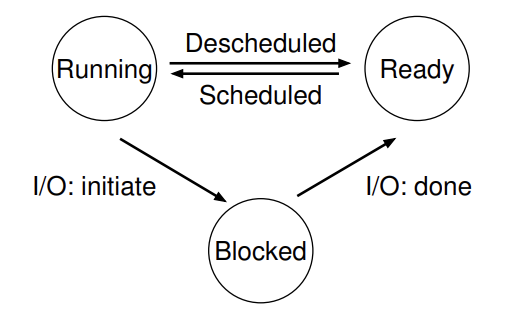
\includegraphics[width=0.4\textwidth]{src/states.png}
    \caption{Estados de un proceso}
\end{figure}

Como se puede ver en el diagrama, un proceso puede moverse entre los estados de \textbf{listo} y \textbf{en ejecución} a discreción del sistema operativo. Ser movido de listo a en ejecución significa que el proceso ha sido \textit{planificado}; ser movido de en ejecución a listo significa que el proceso ha sido \textit{desplanificado}. Una vez que un proceso se ha bloqueado (por ejemplo, al iniciar una operación de entrada/salida), el sistema operativo lo mantendrá en ese estado hasta que ocurra algún evento (por ejemplo, la finalización de la operación de I/O); en ese momento, el proceso pasa nuevamente al estado listo (y potencialmente inmediatamente al estado de ejecución, si el sistema operativo así lo decide).

\subsection{Estructuras de control de procesos}
En resumen, el sistema operativo (SO) necesita conocer en todo momento el estado de los recursos administrados y el de todos los procesos del sistema. Con respecto a los recursos, el SO debe conocer el estado de: \textit{Memoria, Dispositivos de E/S y Sistema de archivos}

Los sistemas operativos están llenos de diversas estructuras de datos importantes, la lista de procesos es la primera de estas estructuras. Es una de las más simples, pero ciertamente cualquier sistema operativo que tenga la capacidad de ejecutar múltiples programas a la vez tendrá algo similar a esta estructura para hacer un seguimiento de todos los programas en ejecución en el sistema.

\subsection{Creación de procesos en sistemas Unix}
\subsubsection{Llamada al sistema \texttt{fork()}}
La llamada al sistema \texttt{fork()} es una de las operaciones fundamentales en sistemas operativos UNIX y similares. Su función principal es crear un nuevo proceso duplicando el proceso que la llamó. El proceso original se conoce como el "proceso padre", mientras que el nuevo proceso creado se llama "proceso hijo". Ambos procesos continúan ejecutándose desde la línea donde se llamó a \texttt{fork()}, pero con una diferencia clave en su comportamiento debido al valor de retorno de \texttt{fork()}. Por ejemplo, veamos el siguiente código:

\begin{verbatim}
#include <stdio.h>
#include <stdlib.h>
#include <unistd.h>

int main(int argc, char *argv[]) {
    printf("hello (pid:%d)\n", (int) getpid());
    int rc = fork();
    if (rc < 0) {
        // fork failed
        fprintf(stderr, "fork failed\n");
        exit(1);
    } else if (rc == 0) {
        // child (new process)
        printf("child (pid:%d)\n", (int) getpid());
    } else {
        // parent goes down this path (main)
        printf("parent of %d (pid:%d)\n",
        rc, (int) getpid());
    }
    return 0;
}
\end{verbatim}

\footnote{OSTEP, Cap.5, La API de los Procesos}

Se puede ver que antes de llamar a \texttt{fork()}, el proceso padre imprime su PID. Luego, después de llamar a \texttt{fork()}, el proceso hijo imprime su PID y el proceso padre imprime el PID del proceso hijo. La salida de este programa se verá algo así:

\begin{verbatim}
hello (pid:1234)
parent of 1235 (pid:1234)
child (pid:1235)
\end{verbatim}

Pero ¿cómo funciona \textit{fork()}? si fork falla retorna un valor negativo, en este caso el programa imprimirá un mensaje de error y terminará. Si \textit{fork()} tiene éxito, se devolverá dos veces, una vez en el proceso padre y otra en el proceso hijo. En el proceso hijo, el valor devuelto será 0, mientras que en el proceso padre, el valor devuelto será el PID del proceso hijo. Esto es lo que permite que el programa diferencie entre el proceso padre y el proceso hijo.

\begin{summary}{Resumen}
    Con esto concluimos que, luego de llamar a \texttt{fork()} se crea un nuevo proceso hijo, el cual es una copia exacta del proceso padre. Lo que se clona es lo siguiente:
    \begin{itemize}
        \item Program Text: El código máquina del programa.
        \item Stack: Las variables locales y los argumentos de la función.
        \item PCB: El PCB del proceso.
        \item Data: Las variables globales.
    \end{itemize}
\end{summary}

Este comportamiento es esencial para operaciones de multitarea y creación de nuevos procesos en sistemas UNIX, y es la base sobre la que se construyen muchas otras operaciones del sistema operativo.

\footnote{Pablo Martínez - SO1 Prácticos 2021- FCEFyN - UNC}
Veamos ahora otro código:
\begin{verbatim}
#include <stdio.h>
#include <stdlib.h>
#include <unistd.h>
int main (int argc, char *argv[]) {
    pid_t childpid = 0;
    int i, n;
    if (argc != 2){ /* check for valid number of command-line arguments */
        fprintf(stderr, "Usage: %s processes\n", argv[0]);
        return 1;
    }
    n = atoi(argv[1]);
    for (i = 1; i < n; i++){
        if (childpid = fork())
        break;
    }
    fprintf(stderr, "i:%d process ID:%ld parent ID:%ld child ID:%ld\n",
    i, (long)getpid(), (long)getppid(), (long)childpid);
    return 0;
}
\end{verbatim}

\footnote{Unix Systems Programming: Communication, Concurrency, and Threads - Sec 3.3}
Este programa toma un argumento de línea de comandos que indica cuántos procesos se deben crear. Luego, crea \texttt{n} procesos, cada uno de los cuales imprime su PID, el PID de su padre y el PID de su hijo. La salida de este programa se verá algo así:

\begin{verbatim}
i:1 process ID:1234 parent ID:1233 child ID:1235
i:2 process ID:1235 parent ID:1234 child ID:1236
i:3 process ID:1236 parent ID:1235 child ID:1237
i:4 process ID:1237 parent ID:1236 child ID:1238
\end{verbatim}

Graficamente se puede ver como funciona la llamada a \texttt{fork()} en el siguiente diagrama:

\begin{figure}[h]
    \centering
    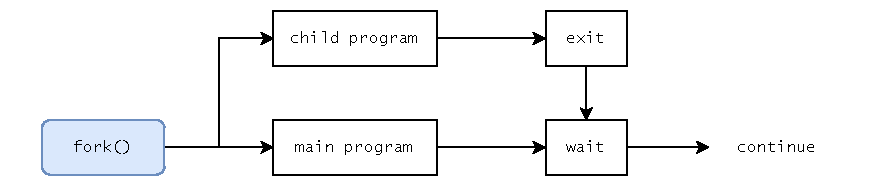
\includegraphics[width=0.9\textwidth]{src/fork.pdf}
    \caption{Diagrama de la llamada a \texttt{fork()}}
\end{figure}

Cabe destacar que el hijo no es una copia exacta. Específicamente, aunque ahora tiene su propia copia del espacio de direcciones (es decir, su propia memoria privada), sus propios registros, su propio contador de programa (PC), y demás, el valor que devuelve al que llamó a fork() es diferente. En particular, mientras que el padre recibe el PID del hijo recién creado, el hijo recibe un código de retorno de cero. Esta diferenciación es útil porque facilita escribir el código que maneja los dos casos diferentes.

Se puede notar en el diagrama una nueva llamada de espera \texttt{wait()} que se encarga de esperar a que el proceso hijo termine. Si no se llama a \texttt{wait()} el proceso hijo se convierte en un proceso huérfano, es decir, un proceso que no tiene padre. La vemos a continuación.

\subsubsection{Llamada al sistema \texttt{wait()}}
Hasta ahora, solo creamos un proceso hijo que imprime un mensaje y termina. A veces, resulta bastante útil que un proceso padre espere a que un proceso hijo termine lo que está haciendo. Esta tarea se realiza con la llamada al sistema \texttt{wait()}.

En el ejemplo anterior se puede ver que el proceso padre imprime su PID, luego crea un proceso hijo que imprime su PID y el PID del proceso padre. Pero, ¿qué pasa si el proceso hijo no termina inmediatamente? ¿Qué pasa si el proceso hijo realiza un trabajo que lleva tiempo? En este caso, el proceso padre puede esperar a que el proceso hijo termine. Esto se logra con la llamada al sistema \texttt{wait()}. Volvamos ahora para ver esto a otra versión del primer ejemplo:

\begin{verbatim}
#include <stdio.h>
#include <stdlib.h>
#include <unistd.h>
#include <sys/wait.h>

int main(int argc, char *argv[]) {
    printf("hello (pid:%d)\n", (int) getpid());
    int rc = fork();
    if (rc < 0) { // fork failed; exit
        fprintf(stderr, "fork failed\n");
        exit(1);
    } else if (rc == 0) { // child (new process)
        printf("child (pid:%d)\n", (int) getpid());
    } else { // parent goes down this path
        int rc_wait = wait(NULL);
        printf("parent of %d (rc_wait:%d) (pid:%d)\n",
        rc, rc_wait, (int) getpid());
    }
    return 0;
}
\end{verbatim}

\footnote{OSTEP, Cap.5, La API de los Procesos}

En este caso, el proceso padre crea un proceso hijo y luego llama a \texttt{wait()}. La llamada a \texttt{wait()} hace que el proceso padre se bloquee hasta que el proceso hijo termine. Una vez que el proceso hijo termina, el proceso padre se desbloquea y continúa su ejecución. La salida de este programa se verá algo así:

\begin{verbatim}
hello (pid:29266)
child (pid:29267)
parent of 29267 (rc_wait:29267) (pid:29266)
\end{verbatim}

\footnote{Pablo Martínez - SO1 Prácticos 2021- FCEFyN - UNC}

\subsubsection{Llamada al sistema \texttt{exec()}}

La familia de funciones \texttt{exec()} reemplaza la imagen del proceso actual con una nueva imagen de proceso. Cuando un programa llama a una función exec, ese proceso deja de ejecutar el programa actual inmediatamente y comienza a ejecutar un nuevo programa desde el principio.

\begin{mdframed}[backgroundcolor=gray!10]
Debido a que exec reemplaza el programa que hace la llamada con otro, nunca regresa, a menos que ocurra un error.
\end{mdframed}

Es decir, que si un programa llama a una función exec, el programa actual se detiene y se carga un nuevo programa en su lugar. Por lo tanto, si la llamada a exec tiene éxito, el programa que la llamó nunca regresará. Si la llamada a exec falla, el programa que la llamó continuará ejecutándose como si nada hubiera pasado. Lo que hace es: dado el nombre de un ejecutable (por ejemplo, wc), y algunos argumentos (por ejemplo, test.c), carga el código de ese ejecutable y sobrescribe su segmento de código actual con él; el \textit{stack}, el \textit{heap} y otras partes del espacio de memoria del programa se reinicializan. Luego, el sistema operativo simplemente ejecuta ese programa, pasando los argumentos como el argv de ese proceso. Así, no crea un nuevo proceso; más bien, transforma el programa que se está ejecutando actualmente en un programa diferente (wc). \footnote{OSTEP, Cap.5, La API de los Procesos}

Ahora bien, ¿por qué es útil esto? Bueno, la llamada a \texttt{exec()} es útil porque permite que un proceso ejecute cualquier programa que desee, no solo el programa que se cargó inicialmente. Por ejemplo, un shell puede ejecutar cualquier programa que desee, simplemente llamando a \texttt{exec()} con el nombre del programa y cualquier argumento que desee pasar a ese programa. Por lo tanto, \texttt{exec()} es una forma de que un proceso cambie de programa a mitad de camino, lo que es útil para muchas aplicaciones.

Existen distintos tipos de llamadas a \texttt{exec()} \footnote{Pablo Martínez - SO1 Prácticos 2021- FCEFyN - UNC}:
\begin{itemize}
    \item[$\looparrowright$] Llamadas que contienen la letra \texttt{p} en su nombre, como \texttt{execlp()} o \texttt{execvp()}, buscan el archivo ejecutable en el \textit{path} del sistema.
    \item[$\looparrowright$] Llamadas que contienen la letra \texttt{l} en su nombre, como \texttt{execl()} o \texttt{execlp()}, requieren que los argumentos del programa se pasen como una lista de argumentos separados por comas.
    \item[$\looparrowright$] Llamadas que contienen la letra \texttt{v} en su nombre, como \texttt{execv()} o \texttt{execvp()}, requieren que los argumentos del programa se pasen como un vector de punteros a cadenas terminadas en \texttt{NULL}.
    \item[$\looparrowright$] Llamadas que contienen la letra \texttt{e} en su nombre, como \texttt{execve()} o \texttt{execvpe()}, aceptan un argumento adicional que especifica el entorno del nuevo programa. El argumento debe ser un array de punteros a cadenas terminadas en \texttt{NULL} donde cada cadena tiene la forma \texttt{nombre=valor}.
\end{itemize}

\subsection{API de Procesos en la shell}
El shell es simplemente un programa de usuario. Muestra un prompt y luego espera que escribas algo en él. Luego, escribes un comando (es decir, el nombre de un programa ejecutable, más cualquier argumento) en él; en la mayoría de los casos, el shell averigua dónde en el sistema de archivos reside el ejecutable, llama a \texttt{fork()} para crear un nuevo proceso hijo para ejecutar el comando, llama a alguna variante de \texttt{exec()} para ejecutar el comando, y luego espera a que el comando termine llamando a \texttt{wait()}. Cuando el proceso hijo termina, el shell retorna de \texttt{wait()} e imprime nuevamente un prompt, listo para tu próximo comando.

La separación de \texttt{fork()} y \texttt{exec()} permite que el shell haga un montón de cosas útiles con bastante facilidad. Por ejemplo:
\begin{verbatim}
$ wc p3.c > newfile.txt
\end{verbatim}

En el ejemplo anterior, la salida del programa \texttt{wc} se redirige al archivo de salida \texttt{newfile.txt}. La forma en que el shell logra esta tarea es bastante simple: cuando se crea el proceso hijo, antes de llamar a \texttt{exec()}, el shell cierra la salida estándar y abre el archivo newfile.txt. Al hacer esto, cualquier salida del programa que está a punto de ejecutarse, wc, se envía al archivo en lugar de a la pantalla.

Aunque el shell es un programa bastante simple, es un buen ejemplo de cómo se pueden combinar las llamadas al sistema \texttt{fork()}, \texttt{exec()} y \texttt{wait()} para hacer cosas bastante útiles. Hay muchas formas de combinar las llamadas al sistema para lograr diferentes comportamientos, y el shell es un buen ejemplo de cómo se pueden combinar las llamadas al sistema para lograr un manejo de procesos bastante sofisticado.

\subsubsection{Redirecciones de E/S}
La mayoría de las operaciones de E/S de archivos en un sistema UNIX se pueden realizar utilizando solo cinco funciones: open, read, write, lseek y close. Luego se puede analizar el efecto de varios tamaños de buffer en las funciones de lectura y escritura. Estas funciones menudo se denominan E/S sin buffer, en contraste con las rutinas de E/S estándar. El término sin buffer significa que cada operación de lectura o escritura invoca una llamada al sistema en el kernel. Estas funciones de E/S sin buffer no forman parte de ISO C, pero sí son parte de POSIX.1 y la Especificación Única de UNIX. \footnote{Advanced Programming in the UNIX Environment - Cap.3}

\subsubsection{File Descriptors}
Para el kernel, todos los archivos abiertos se identifican mediante descriptores de archivos. Un descriptor de archivo es un número entero no negativo. Cuando abrimos un archivo existente o creamos un archivo nuevo, el kernel devuelve un descriptor de archivo al proceso. Cuando queremos leer o escribir en un archivo, identificamos el archivo con el descriptor de archivo que fue devuelto por open o creat como argumento para las funciones read o write.

Por convención, las shells del sistema UNIX asocian el descriptor de archivo 0 con la entrada estándar de un proceso, el descriptor de archivo 1 con la salida estándar y el descriptor de archivo 2 con el error estándar. 

\begin{summary}{Convenciones de los descriptores de archivo}
    Aunque sus valores están estandarizados por POSIX.1, los números 0, 1 y 2 deben ser reemplazados en aplicaciones compatibles con POSIX por las constantes simbólicas \texttt{STDIN\_FILENO}, \texttt{STDOUT\_FILENO} y \texttt{STDERR\_FILENO} para mejorar la legibilidad. Estas constantes están definidas en el archivo de cabecera $<$unistd.h$>$.
\end{summary}

\subsubsection{Función \texttt{open()}}
Un archivo se abre o se crea llamando a la función open:
\begin{lstlisting}[language=C]
    int open(const char *pathname, int flags);
    int open(const char *pathname, int flags, mode_t mode);
\end{lstlisting}
Ambas devuelven: descriptor de archivo si todo está bien, -1 en caso de error.

\begin{enumerate}
    \item El parámetro path es el nombre del archivo que se va a abrir o crear. 
    \item Esta función tiene una multitud de opciones, que se especifican mediante el argumento segundo argumento flag. Este argumento se forma combinando con OR:
    \begin{itemize}
        \item \textbf{O\_RDONLY}: Abrir solo para lectura.
        \item \textbf{O\_WRONLY}: Abrir solo para escritura.
        \item \textbf{O\_RDWR}: Abrir para lectura y escritura.
    \end{itemize}
    La mayoría de las implementaciones definen \texttt{O\_RDONLY} como 0, \texttt{O\_WRONLY} como 1 y \texttt{O\_RDWR} como 2.
    \begin{itemize}
        \item \textbf{O\_EXEC}: Abrir solo para ejecutar.
        \item \textbf{O\_SEARCH}: Abrir solo para buscar (aplica a directorios).
    \end{itemize}
    \textit{De estos cinco, solo uno debe especificarse.} Los siguientes flags son opcionales:
    \begin{itemize}
        \item \textbf{O\_APPEND}: Añadir al final del archivo en cada escritura.
        \item \textbf{O\_CLOEXEC}: Configurar la bandera FD\_CLOEXEC del descriptor de archivo. 
        \item \textbf{O\_CREAT}: Crear el archivo si no existe. Esta opción requiere un tercer argumento en la función open (un cuarto argumento en la función openat), el mode, que especifica los bits de permisos de acceso del nuevo archivo.
        \item \textbf{O\_DIRECTORY}: Generar un error si el path no refiere a un directorio.
        \item \textbf{O\_EXCL}: Generar un error si también se especifica O\_CREAT y el archivo ya existe. Esta verificación de si el archivo ya existe y la creación del archivo si no existe es una operación atómica. 
        \item \textbf{O\_NOCTTY}: Si el path refiere a un dispositivo terminal, no asignar el dispositivo como terminal de control para este proceso.
        \item \textbf{O\_NOFOLLOW}: Generar un error si el path refiere a un enlace simbólico.
        \item \textbf{O\_NONBLOCK}: Si el path refiere a un FIFO, archivo especial de bloque o archivo especial de carácter, esta opción establece el modo no bloqueante para la apertura del archivo y la E/S posterior. 
    \end{itemize} \footnote{Advanced Programming in the UNIX Environment - Cap.3}
\end{enumerate}

\subsubsection{Función \texttt{close()}}
La función close cierra un descriptor de archivo:
\begin{lstlisting}[language=C]
    int close(int fd);
\end{lstlisting}
Devuelve 0 si todo está bien, -1 en caso de error. Se encarga de cerrar un archivo también libera cualquier bloqueo de registro que el proceso pueda tener sobre el archivo.

\subsubsection{Función \texttt{read()}}
La función read lee datos de un archivo abierto:
\begin{lstlisting}[language=C]
    ssize_t read(int fd, void *buf, size_t count);
\end{lstlisting}
Devuelve el número de bytes leídos, 0 si se alcanza el final del archivo, -1 en caso de error.

Los argumentos que toman hacen referencia a:
\begin{itemize}
    \item \textbf{fd}: Descriptor de archivo.
    \item \textbf{buf}: Buffer donde se almacenarán los datos leídos.
    \item \textbf{count}: Número de bytes a leer.
\end{itemize}
La salida de error se encargará del mal manejo de los argumentos, es decir si se le pasa un descriptor cerrado, un buf inválido o un count negativo, en esos casos simplemente devolverá -1.

Si la función recibe mas bytes que los disponibles, la función devolverá el número de bytes disponibles. Si se llega al final del archivo, la función en la siguiente llamada devolverá 0.

\subsubsection{Función \texttt{write()}}
La función write escribe datos en un archivo abierto:
\begin{lstlisting}[language=C]
    ssize_t write(int fd, const void *buf, size_t count);
\end{lstlisting}
Devuelve el número de bytes escritos, -1 en caso de error. Es decir, generalmente el valor de retorno es igual al argumento count, pero si se produce un error, el valor de retorno es -1. Una causa normal de error es que el disco esté lleno.

\subsection{File Sharing}
Un sistema UNIX soporta la compartición de archivos entre procesos. Para poder entender mas este suceso, es necesario examinar algunas estructuras del kernel asociadas a los archivos.
\begin{enumerate}
    \item Cada proceso tiene una \textbf{tabla de descriptores de archivos} (file descriptor table) que contiene lo siguiente:
    \begin{itemize}
        \item Los flags de archivo,
        \item Un puntero a la entrada de la tabla de archivos del archivo en el kernel.
    \end{itemize}
    \item El kernel mantiene una \textbf{tabla de archivos} (file table) que contiene lo siguiente:
    \begin{itemize}
        \item Flags de estado del archivo,
        \item Offset de archivo (la posición actual del archivo),
        \item Puntero a la estructura de v-node del archivo.
    \end{itemize}
    \item Una estructura de \textbf{v-node} (v-node structure) : es parte de la abstracción que permite a los sistemas operativos manejar múltiples tipos de sistemas de archivos, contiene lo siguiente:
    \begin{itemize}
        \item Información vnode,
        \item Información inode, almacena metadatos del archivo (por ejemplo, tamaño, propietario, permisos, etc.).
    \end{itemize}
\end{enumerate}

Visualmente podemos ver a un proceso con dos archivos abiertos en la siguiente figura:

\begin{figure}[h]
    \centering
    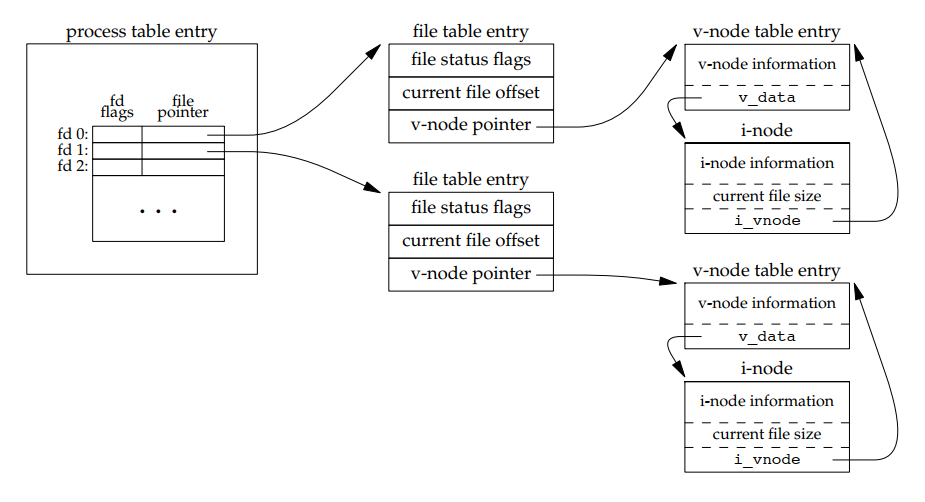
\includegraphics[width=0.8\textwidth]{src/filesharing.png}
    \caption{Files in processes}
\end{figure}

Ahora bien, si dos procesos comparten el mismo archivo no quiere decir que compartan la tabla de archivos. Una razón por la que cada proceso tiene su propia entrada en la tabla de archivos es para que cada uno tenga su propio desplazamiento actual en el archivo.

\begin{figure}[h]
    \centering
    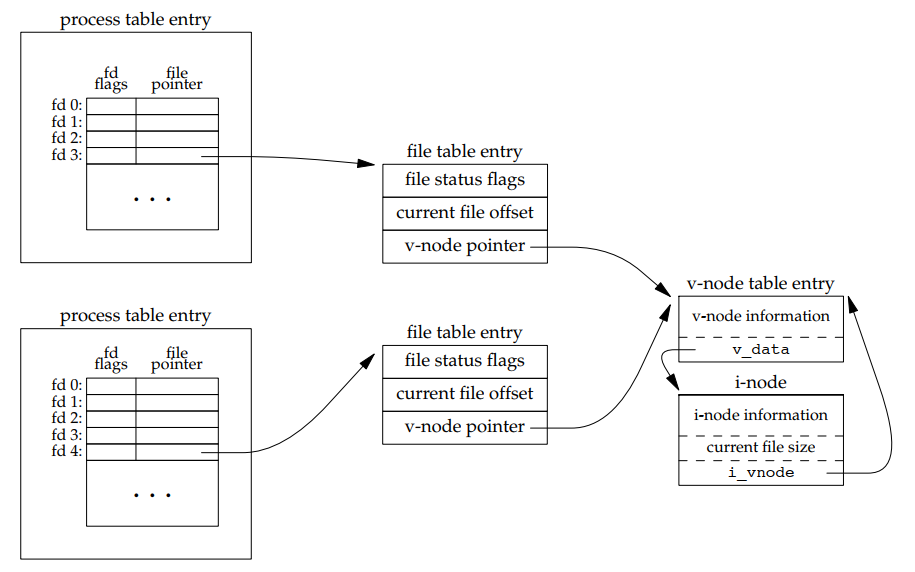
\includegraphics[width=0.7\textwidth]{src/filesharing2.png}
    \caption{File Sharing}
\end{figure}

Pero es necesario también tener en cuenta como se maneja el offset con las funciones de E/S:
\begin{itemize}
    \item Después de que cada escritura se completa mediante la función \texttt{write()}, el offset actual del archivo en la entrada de la tabla de archivos se incrementa en el número de bytes escritos. Si esto hace que el desplazamiento actual del archivo exceda el tamaño actual del archivo, el tamaño del archivo en la entrada de la tabla de i-nodes se ajusta al desplazamiento actual del archivo.
    \item Si un archivo se abre con la flag \texttt{O\_APPEND}, se establece una flag correspondiente en los flags de estado del archivo en la entrada de la tabla de archivos. Cada vez que se realiza una escritura en un archivo con esta flag de append activada, el desplazamiento actual del archivo en la tabla de archivos se establece primero en el tamaño actual del archivo, obtenido de la tabla de i-nodes. Esto fuerza que cada escritura se agregue al final actual del archivo.
    \item Si un archivo se posiciona al final actual del archivo usando lseek, todo lo que sucede es que el desplazamiento actual del archivo en la tabla de archivos se ajusta al tamaño actual del archivo, obtenido de la entrada de la tabla de i-nodes. 
\end{itemize}

\begin{summary}{Comportamiento con fork, dup}
    Es posible que mas de un file descriptor apunte a la misma entrada de la tabla de archivos:
    \begin{itemize}
        \item Por ejemplo, si un proceso llama a \texttt{fork()} después de abrir un archivo, el proceso hijo hereda la tabla de descriptores de archivos del proceso padre, incluido el descriptor de archivo abierto. Si el proceso hijo o el proceso padre cierran el descriptor de archivo, el archivo se cierra para ambos procesos. Si el proceso hijo o el proceso padre cambian el desplazamiento actual del archivo, el cambio se refleja en ambos procesos.
        \item Cuando se llama a dup o dup2, se crea un nuevo descriptor de archivo que apunta a la misma entrada de la tabla de archivos que el descriptor de archivo original. Si se cierra uno de los descriptores de archivo, el archivo permanece abierto hasta que se cierre el otro descriptor de archivo.
    \end{itemize}
\end{summary}

\subsubsection{Funciones \texttt{dup} y \texttt{dup2}}
Un file descriptor abierto puede ser duplicado con la función \texttt{dup} o \texttt{dup2}:
\begin{lstlisting}[language=C]
    int dup(int oldfd);                  int dup2(int oldfd, int newfd);
\end{lstlisting}
El \texttt{file descriptor} devuelto por la función \texttt{dup} es el descriptor de archivo más bajo que no está en uso. En cambio con \texttt{dup2()} especificamos el valor del nuevo descriptor con el argumento \texttt{newfd}. Acá hay algunas decisiones que se deben tener en cuenta:
\begin{enumerate}
    \item Si \texttt{newfd} es un descriptor de archivo abierto, primero se cierra.
    \item Si \texttt{newfd} es igual a \texttt{oldfd}, \texttt{dup2()} devuelve \texttt{newfd} sin cerrar nada.
    \item En caso contrario, el flag del descriptor de archivo \texttt{FD\_CLOEXEC} se borra en el nuevo descriptor de archivo.
\end{enumerate} 

Por ejemplo, supongamos que se ejecuta la línea \texttt{newfd = dup(1)}, como el sistema tiene abiertos los descriptores 0, 1 y 2, el nuevo descriptor devuelto será 3. Y ambos apuntarán a la misma entrada de la tabla de archivos, compartiendo sus flags y offset.

\begin{figure}[h]
    \centering
    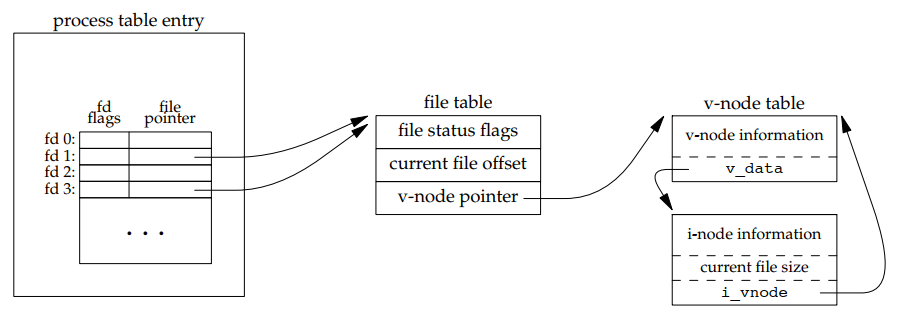
\includegraphics[width=0.7\textwidth]{src/dupdata.png}
    \caption{Función \texttt{dup}}
\end{figure}

\begin{summary}{Observaciones}
    El sistema operativo cuando libera un file descriptor, lo deja libre para su uso, es decir si por ejemplo cerramos la entrada estándar (descriptor 0), el próximo file descriptor que se abra será el 0. Por otro lado, si se llama a \texttt{dup()} o \texttt{dup2()} se crea un nuevo file descriptor que apunta a la misma entrada de la tabla de archivos que el descriptor de archivo original. Si se cierra uno de los descriptores de archivo, el archivo permanece abierto hasta que se cierre el otro descriptor de archivo.
\end{summary}


\newpage
\section{Ejecución directa limitada}

Como ya habia mencionado al principio, un sistema operativo debe ser capaz de ejecutar múltiples programas a la vez. Pero, ¿cómo se logra esto? una de las técnicas más simples para lograr esto es la \textbf{ejecución directa limitada}. En este modelo, el sistema operativo simplemente alterna la ejecución de los programas, permitiendo que cada uno se ejecute durante un tiempo limitado antes de pasar al siguiente.

¿A que llamamos ejecución directa? La parte de “ejecución directa” de la idea es simple: simplemente ejecuta el programa directamente en la CPU. Así, cuando el sistema operativo desea iniciar la ejecución de un programa, crea una entrada para él en la lista de procesos, asigna algo de memoria, carga el código del programa en la memoria (desde el disco), localiza su punto de entrada, salta a él y comienza a ejecutar el código del usuario.

\begin{figure}[h]
    \centering
    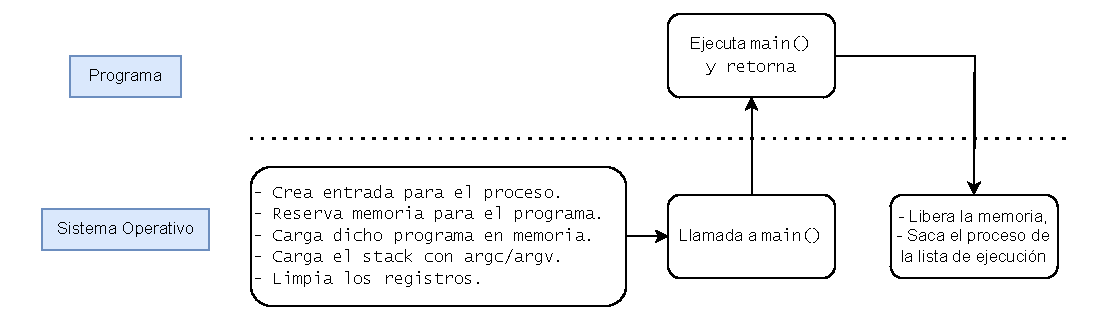
\includegraphics[width=0.9\textwidth]{src/edl.pdf}
    \caption{Ejecución directa limitada}
\end{figure} \footnote{OSTEP, Cap.6, Ejecución Directa Limitada}

Este enfoque da lugar a algunos problemas en nuestra búsqueda de \textit{virtualizar la CPU}. El primero es sencillo: si simplemente ejecutamos un programa, \textbf{¿cómo puede el sistema operativo asegurarse de que el programa no haga nada que no queramos que haga, y al mismo tiempo lo ejecute de manera eficiente?} El segundo: cuando estamos ejecutando un proceso, \textbf{¿cómo detiene el sistema operativo su ejecución y cambia a otro proceso, implementando así el reparto de tiempo que necesitamos para virtualizar la CPU?}

\subsection{Problema 1 - Operaciones privilegiadas}
El primer problema es que el sistema operativo no quiere que los programas de usuario hagan cualquier cosa que quieran. Por ejemplo, no queremos que un programa de usuario pueda leer o escribir en cualquier parte de la memoria, o que pueda leer o escribir en cualquier archivo en el disco. En cambio, queremos que los programas de usuario se ejecuten en un modo restringido, donde solo pueden hacer cosas que el sistema operativo les permite hacer. A este modo restringido se le llama \textbf{modo usuario}. Por otro lado, el sistema operativo se ejecuta en un modo más privilegiado, llamado \textbf{modo kernel}. En este modo, el sistema operativo puede hacer cualquier cosa que desee, como leer y escribir en cualquier parte de la memoria, leer y escribir en cualquier archivo en el disco, y más.

\begin{mdframed}[backgroundcolor=gray!10]
    En resumen, el enfoque que tomamos es introducir un nuevo modo del procesador, conocido como \textit{modo usuario}; el código que se ejecuta en modo usuario tiene restricciones sobre lo que puede hacer. Por otro lado, está el \textit{modo kernel}, en el cual se ejecuta el sistema operativo. En este modo, el código que se ejecuta puede hacer lo que quiera, incluyendo operaciones privilegiadas como emitir solicitudes de E/S y ejecutar todo tipo de instrucciones restringidas.
\end{mdframed}

Sin embargo, aún nos queda una incógnita ¿qué debe hacer un proceso de usuario cuando desea realizar algún tipo de operación privilegiada, como leer desde el disco? Para habilitar esto, prácticamente todo el hardware moderno proporciona la capacidad para que los programas de usuario realicen una llamada al sistema.

\subsubsection{Ejecución de una \texttt{syscall}}
Para ejecutar una llamada al sistema, un programa debe ejecutar una instrucción especial de trampa (trap). Esta instrucción simultáneamente salta al kernel y eleva el nivel de privilegio al modo kernel; una vez en el kernel, el sistema puede realizar las operaciones privilegiadas necesarias (si están permitidas) y, por lo tanto, hacer el trabajo requerido para el proceso que llamó. Cuando termina, el sistema operativo ejecuta una instrucción especial de retorno de trampa, que regresa al programa de usuario que llamó mientras simultáneamente reduce el nivel de privilegio de vuelta al modo usuario.

\newpage
\begin{figure}[h]
    \centering
    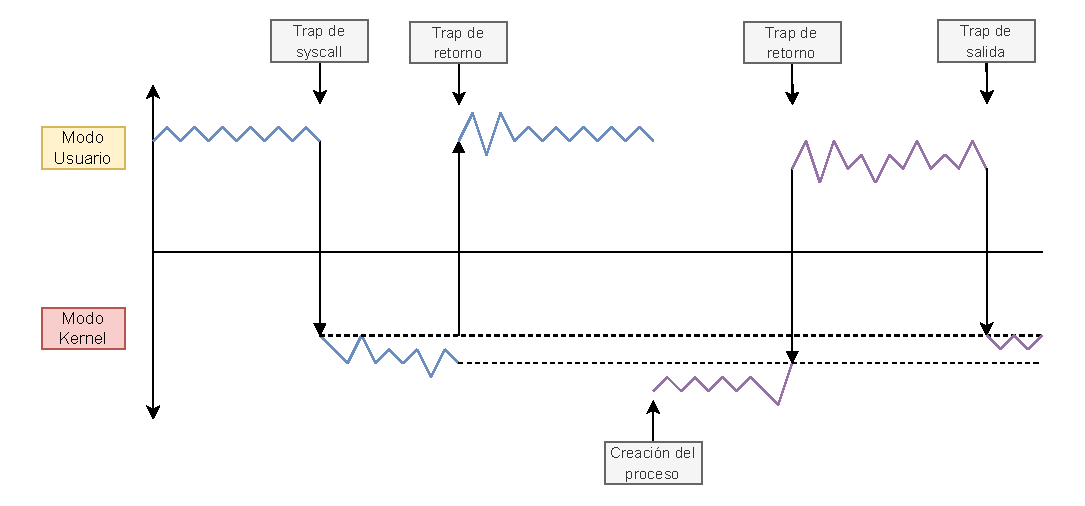
\includegraphics[width=1\textwidth]{src/syscall.pdf}
    \caption{Ejecución de una \texttt{syscall}}
\end{figure} \footnote{OSTEP, Cap.6, Ejecución Directa Limitada}

Hay un detalle importante que se dejó fuera de esta discusión: ¿cómo sabe la trampa qué código ejecutar dentro del sistema operativo? Claramente, el proceso que llama no puede especificar una dirección a la cual saltar (como lo harías al hacer una llamada a un procedimiento); hacerlo permitiría que los programas saltaran a cualquier parte del kernel, lo cual claramente es una "Muy Mala Idea". Por lo tanto, el kernel debe controlar cuidadosamente qué código se ejecuta al ocurrir una trampa.

Una buena idea es agregar un nivel mas de indirección, las llamadas \textbf{trap tables}, cuando la máquina se inicia, lo hace en modo kernel y, por lo tanto, es libre de configurar el hardware de la máquina según sea necesario. Una de las primeras cosas que hace el sistema operativo es decirle al hardware qué código ejecutar cuando ocurren ciertos eventos excepcionales. Por ejemplo cuando ocurre una trampa, el sistema operativo configura la trampa para saltar a una dirección específica en la memoria, donde reside el código del kernel que maneja esa trampa en particular. De esta manera, cuando ocurre una trampa, el hardware salta a la dirección de la trampa, y el kernel se ejecuta en modo kernel, listo para manejar la trampa.

La trap table, la define el sistema operativo, pero la usa el hardware. El sistema operativo informa al hardware de las ubicaciones de estos \textbf{trap handlers}, generalmente con algún tipo de instrucción especial. Una vez que el hardware está informado, recuerda la ubicación de estos manejadores hasta que la máquina se reinicia nuevamente, y así el hardware sabe qué hacer (es decir, a qué código saltar) cuando se producen llamadas al sistema y otros eventos excepcionales.

\subsubsection{Fases de ejecución directa limitada}
En resumen, la ejecución directa limitada se puede dividir en las siguientes fases:
\begin{itemize}
    \item \textbf{Booteo:} Se inicializa la \textbf{trap table} y se configura el hardware para que se ejecute en modo kernel.
    \item \textbf{Ejecución:} Aca se crea la entrada a la lista de procesos, junto con la asignación de memoria y la carga del código del programa en la memoria. Luego se ejecuta el código del usuario en modo usuario.
\end{itemize}
Esto es muy por encima de lo que realmente sucede, pero es un buen punto de partida para comprender cómo se ejecutan los programas en un sistema operativo moderno. En el siguiente gráfico se puede ver con mas profundidad el efecto:
\newpage
\begin{figure}[h]
    \centering
    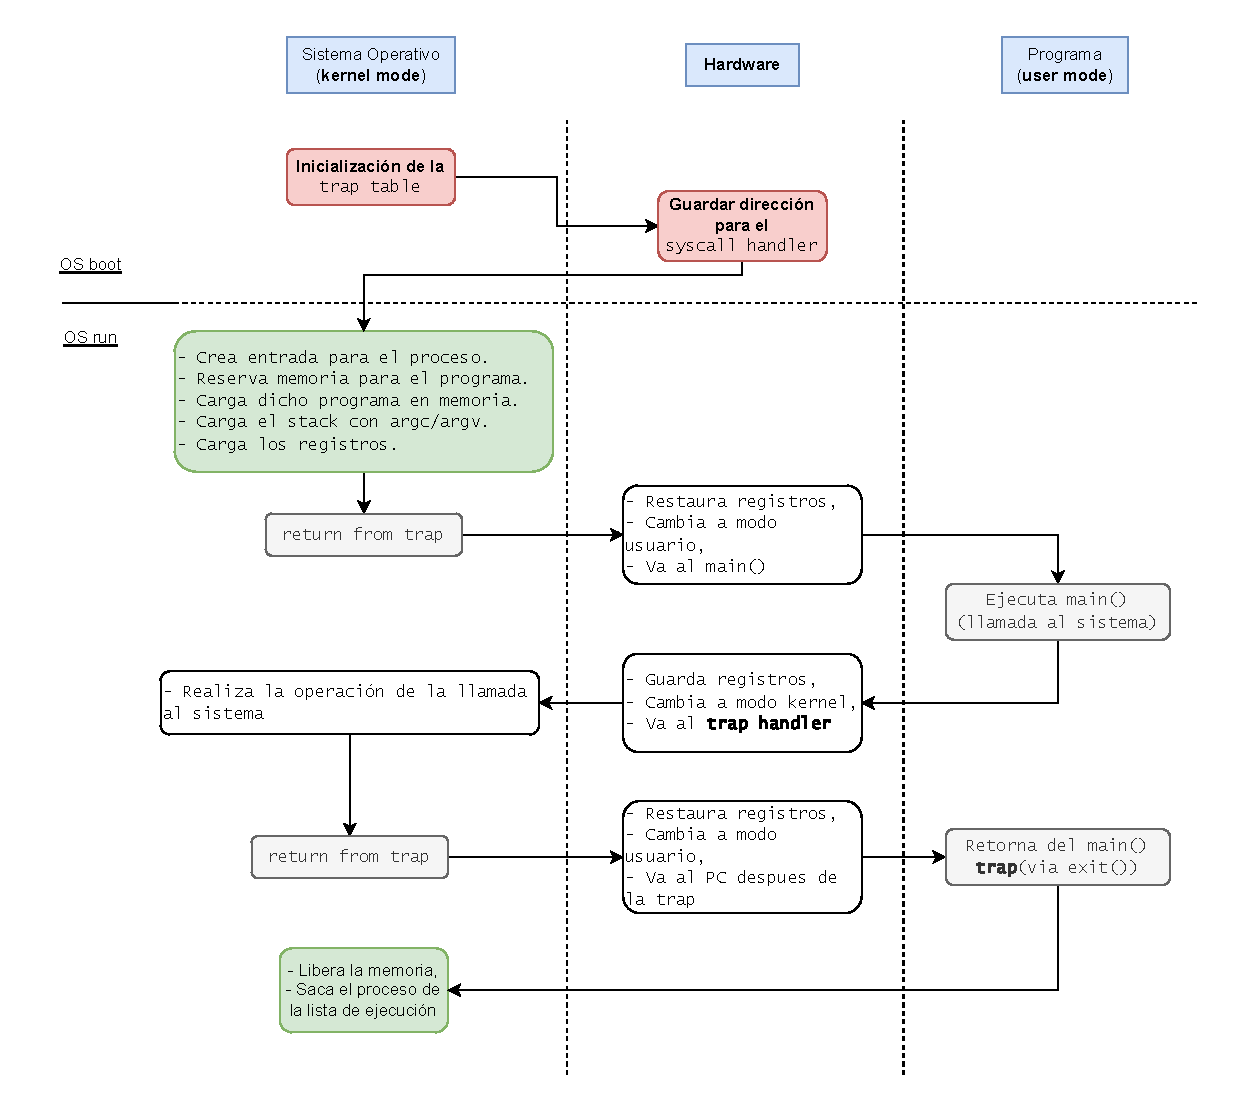
\includegraphics[width=1\textwidth]{src/edl2.pdf}
    \caption{Ejecución directa limitada}
\end{figure} \footnote{OSTEP, Cap.6, Ejecución Directa Limitada}

Los puntos mas importantes de la ejecución directa limitada son:
\begin{itemize}
    \item \textbf{Inicialización trap table}: Durante el arranque del sistema operativo, se inicializa la "trap table". Esta tabla contiene direcciones de manejadores de interrupciones, incluyendo el manejador de llamadas al sistema (syscall handler). Estos manejadores son funciones en el kernel que son llamadas cuando se produce una interrupción o una llamada al sistema.
    \item \textbf{Crear entrada para el proceso}: Se crea una entrada para el proceso en la lista de procesos del sistema operativo.
    \item \textbf{Carga y asignación de memoria}: Se asigna memoria para el proceso y se carga el código del programa en la memoria.
    \item \textbf{Carga el stack con argc y argv}: Se carga el stack con los argumentos del programa.
    \item \textbf{Limpia los registros:} Se llena la pila del kernel con los valores iniciales de los registros junto con la dirección de retorno (PC).
    \item \textbf{Return from trap}: Se ejecuta la instrucción de retorno de trampa, que cambia el modo de ejecución de kernel a usuario.
    \item \textbf{Ejecución del programa}: Se ejecuta el código del programa en modo usuario.
    \item \textbf{Handle trap:} cuando el kernel recibe la \textbf{trap} sucede lo siguiente: se guardan los registros del proceso, se cambia el modo de ejecución a kernel, se ejecuta el manejador de la trampa, se restauran los registros del proceso y se ejecuta la instrucción de retorno de trampa.
    \item \textbf{Terminar la ejecución:} El retorno del \texttt{main()} señala el fin de la ejecución del programa, luego se realiza una llamada \texttt{exit()} que genera una trampa y se ejecuta el manejador de la trampa; se libera la memoria asignada al proceso y se elimina la entrada del proceso de la lista de procesos.
\end{itemize}

\subsection{Problema 2 - Cambio de procesos}
El siguiente problema con la ejecucion directa es lograr cambiar de proceso. Un enfoque que algunos sistemas han adoptado en el pasado se conoce como el \textbf{enfoque cooperativo}. En este estilo, el sistema operativo confía en que los procesos del sistema se comporten razonablemente. Se asume que los procesos que se ejecutan durante mucho tiempo cederán periódicamente la CPU para que el sistema operativo pueda decidir ejecutar otra tarea. \footnote{OSTEP, Cap.6, Ejecución Directa Limitada}

\begin{mdframed}[backgroundcolor=gray!10]
    En resumen, el enfoque cooperativo es simple: los procesos se ejecutan hasta que deciden ceder la CPU. En ese momento, el sistema operativo puede decidir ejecutar otro proceso. Este enfoque es simple y fácil de implementar, pero tiene un problema fundamental: si un proceso no cede la CPU, el sistema operativo no puede hacer nada al respecto.
\end{mdframed}

Resulta que la mayoría de los procesos transfieren el control de la CPU al sistema operativo con bastante frecuencia al hacer llamadas al sistema. Los sistemas como este a menudo incluyen una llamada al sistema explícita de \texttt{yield}, que no hace nada excepto transferir el control al sistema operativo para que pueda ejecutar otros procesos. Las aplicaciones también transfieren el control al sistema operativo cuando hacen algo ilegal. Por ejemplo, si una aplicación divide por cero, o intenta acceder a una memoria a la que no debería poder acceder, generará una trampa al sistema operativo. El sistema operativo entonces recuperará el control de la CPU (y probablemente terminará el proceso infractor). \footnote{OSTEP 06 - Clase John Ordoñes}

Esta aproximación demanda de ayuda del hardware, timer interrupts, que son interrupciones que se generan a intervalos regulares. Cuando se produce un timer interrupt, el sistema operativo se despierta y puede decidir si desea cambiar de proceso. Si el sistema operativo decide que es hora de cambiar de proceso, puede hacerlo, y el proceso que estaba en ejecución se detiene y se guarda su estado. Luego, el sistema operativo puede elegir otro proceso para ejecutar, restaurar su estado y comenzar a ejecutarlo.

Una vez se gestiona la interrupción, el \textbf{scheduler} del sistema operativo decide qué proceso se ejecutará a continuación. El scheduler es un componente clave del sistema operativo, y su trabajo es decidir qué proceso se ejecutará a continuación. Hay muchos algoritmos de planificación diferentes que se pueden usar para decidir qué proceso se ejecutará a continuación, y cada uno tiene sus propias ventajas y desventajas.

\subsubsection{Protocolo con timer interrupts}
\begin{summary}{Solución}
Podríamos plantearnos la pregunta de ¿qué sucede cuando un proceso se vuelve malicioso y niega el control del recurso? (es lo que se plantea en los párrafos anteriores), podriamos llamar a los \texttt{timer interrupts} como una función de seguridad integrada en el hardware, que permite al sistema operativo recuperar el control del mismo a intervalos regulares de tiempo, independientemente de si los procesos que utilizan el recurso completaron sus tareas o no. \footnote{CPU Virtualization via Limited Direct Execution - Shivam Mohan}
\end{summary}
Principalmente, el protocolo de cambio de procesos con timer interrupts se puede describir de la siguiente manera:
\begin{enumerate}
    \item Inicializa la \textbf{trap table} y configura el hardware para que se ejecute en modo kernel.
    \item Recordamos las direcciones de los manejadores de interrupciones, incluyendo el manejador de llamadas al sistema.
    \item Inicializamos el timer interrupt y configuramos el hardware para que genere interrupciones a intervalos regulares.
    \item Luego de que transcurra un intervalo de tiempo, se genera un timer interrupt de CPU.
\end{enumerate}

Luego saltamos a un escenario en donde ya hay un proceso en ejecución, el \textbf{proceso A}.

\begin{enumerate}
    \setcounter{enumi}{4}
    \item Se genera una interrupción de temporizador.
    \item Guarda los registros del proceso A en la pila del kernel asociado al proceso A, luego nos movemos al modo kernel y nos movemos al manejador de trampas.
    \item Ahora bien, guardamos los registros del proceso A en una tabla de procesos y tomamos de la tabla de procesos los registros del proceso B y los cargamos en los registros del procesador.
    \item Nos vamos a la pila del kernel asociada al proceso B y salimos de la trampa.
    \item Ahora se restauran los registros del proceso B, nos movemos al \textit{program counter} del proceso B y se ejecuta el proceso B desde el modo usuario.
\end{enumerate}

\begin{figure}[h]
    \centering
    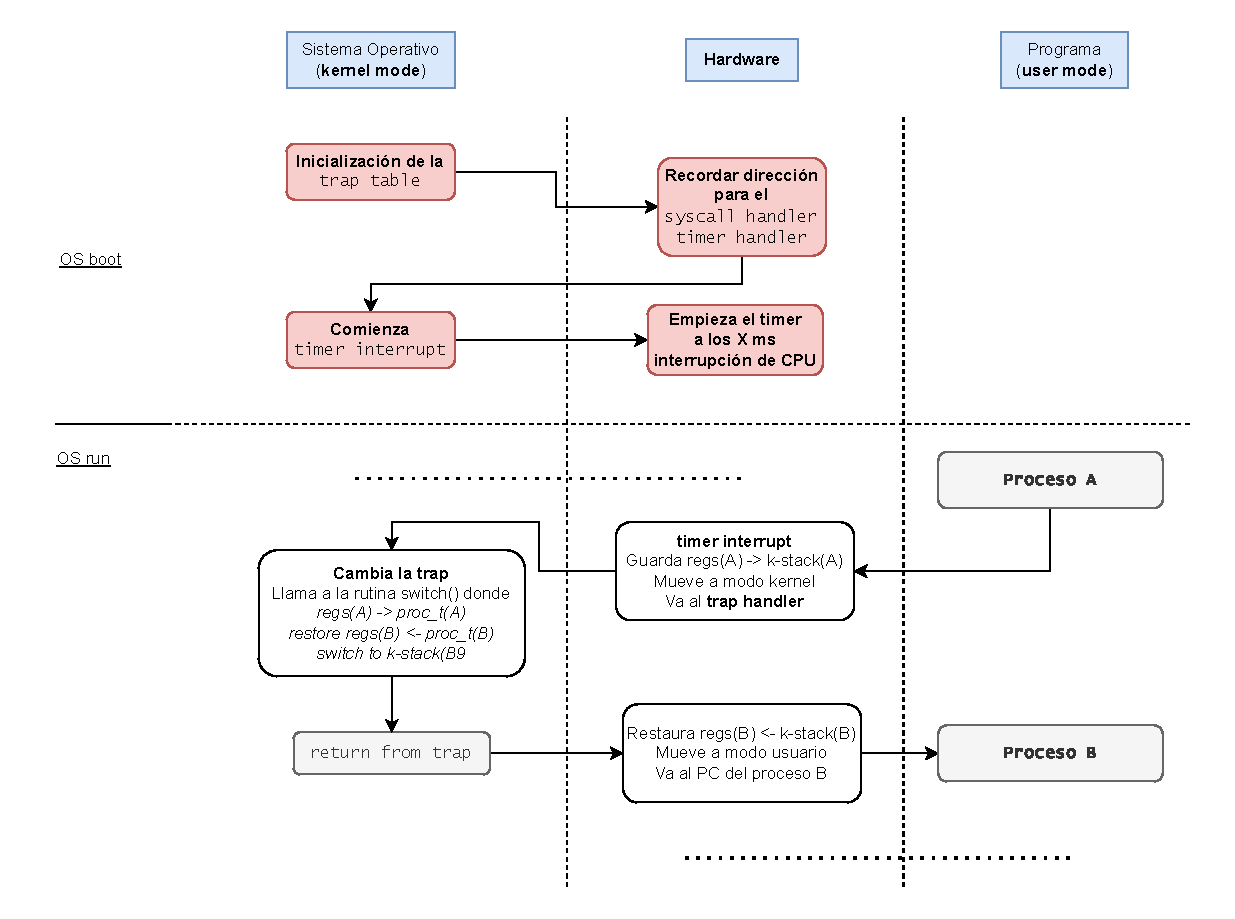
\includegraphics[width=0.9\textwidth]{src/edl3.pdf}
    \caption{Switch de procesos}
\end{figure} \footnote{OSTEP, Cap.6, Ejecución Directa Limitada}

Ahora bien, ¿qué sucede si el proceso estaba en medio de una tarea y se produjo una interrupción y el proceso se vió obligado a liberar recursos? Acá entra el switch de procesos, el \textbf{cambio de contexto}, el cual tiene como idea principal es que cada vez que se le pide a un proceso que renuncie a un recurso que tiene y la tarea del proceso no se completa, el estado actual del proceso (es decir, su contexto) se almacena en la pila del kernel y cada vez que ese proceso recupera el acceso al recurso, el estado se restaura desde la pila del kernel y los procesos pueden continuar la ejecución desde el mismo estado exacto donde lo dejaron antes, de esta manera podemos asegurar que con el tiempo, los procesos puedan lograr un progreso real aunque no tengan acceso al recurso durante todo el tiempo.


\newpage
\section{Planificación}
Las preguntas que surgieron en la sección anterior son: ¿cómo decide el sistema operativo qué proceso se ejecutará a continuación? y con esto llegamos a la \textbf{planificación de procesos}. La planificación de procesos es una de las tareas más importantes de un sistema operativo. El trabajo del planificador es decidir qué proceso se ejecutará a continuación. Hay muchos algoritmos de planificación diferentes que se pueden usar para decidir qué proceso se ejecutará a continuación, y cada uno tiene sus propias ventajas y desventajas.

\begin{definition}
    Un \textbf{algoritmo de planificación} es una estrategia que se utiliza para determinar el orden en que los procesos se ejecutan en un sistema operativo. Debe cumplir con varios objetivos conflictivos: tiempo de respuesta rápido para los procesos, buen rendimiento para trabajos en segundo plano, evitar la inanición de procesos, conciliar las necesidades de procesos de baja y alta prioridad, entre otros. El conjunto de reglas que se utilizan para determinar cuándo y cómo seleccionar un nuevo proceso para ejecutarse se llama \textbf{política de planificación}. \footnote{Understanding the Linux Kernel - Cap.7}
\end{definition}

\begin{definition}
    El tiempo de entrega de un trabajo se define como el momento en que se completa el trabajo menos el momento en que el trabajo llegó al sistema.    
    \begin{equation}
        T_{\text{entrega}} = T_{\text{finalización}} - T_{\text{llegada}}
    \end{equation}
\end{definition}

Como asumimos que todos los trabajos llegan al mismo tiempo, entonces por el momento tenemos que $T_{\text{llegada}} = 0$ y por lo tanto $T_{\text{entrega}} = T_{\text{finalización}}$. Esto irá cambiando a medida que se profundice en el tema.

\subsection{Primero en llegar, primer en salir (FIFO)}

El algoritmo de planificación más simple es el \textbf{primero en llegar, primero en salir (FIFO)}. En este algoritmo, los procesos se ejecutan en el orden en que llegan al sistema. En otras palabras, el sistema operativo mantiene una cola de procesos, y cuando un proceso llega al sistema, se coloca al final de la cola. Cuando el sistema operativo necesita decidir qué proceso se ejecutará a continuación, simplemente toma el primer proceso de la cola y lo ejecuta.

Supongamos que llegan $3$ procesos al sistema, A llegó justo un momento antes que B, que a su vez llegó un momento antes que C. Supongamos también que cada trabajo se ejecuta durante 10 segundos. \footnote{OSTEP, Cap.7, Planificación de Procesos}

\begin{figure}[h]
    \centering
    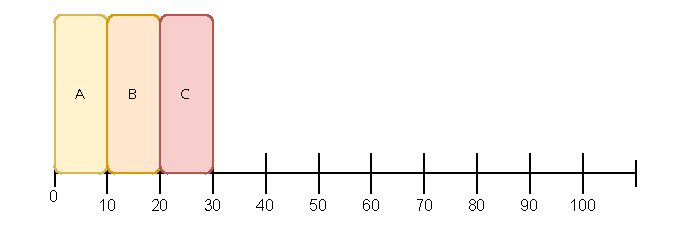
\includegraphics[width=0.9\textwidth]{src/fifo.pdf}
    \caption{Primero en llegar, primero en salir (FIFO)}
\end{figure}

¿Cuál será el tiempo medio de entrega de estos trabajos? se puede ver que A terminó en 10, B en 20 y C en 30. Por lo tanto, el tiempo medio de entrega para los tres trabajos es simplemente $\frac{10+20+30}{3}=20$. Pero esto es porque estamos suponiendo que los trabajos se ejecutan la misma cantidad de tiempo.

Ahora supongamos que el trabajo A corre primero durante 100 segundos completos antes de que B o C tengan la oportunidad de ejecutarse. En este caso el tiempo medio de entrega para los tres trabajos es $\frac{100+110+120}{3}=110$ que es relativamente alto.

\begin{figure}[h]
    \centering
    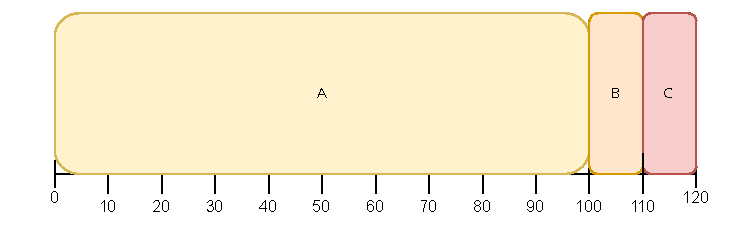
\includegraphics[width=0.9\textwidth]{src/fifo1.pdf}
    \caption{Primero en llegar, primero en salir (FIFO)}
\end{figure}

Este problema se conoce generalmente como el \textbf{efecto de convoy}, en el que una serie de consumidores potenciales de algún recurso, relativamente cortos, se ponen en cola detrás de un consumidor de gran peso. Puede que este escenario de planificación te suene a cuando hay una única fila en un supermercado y lo que sentís cuando ves a la persona en frente tuyo con tres carritos llenos de provisiones, y una chequera en mano; va a demorar un rato.

\subsection{Trabajo mas corto primero (SJF)}

El problema mencionado recien se puede solucionar con el algoritmo de planificación de \textbf{trabajo mas corto primero (SJF)}. En este algoritmo, el sistema operativo elige el proceso que se ejecutará a continuación en función de cuánto tiempo se espera que dure el proceso. En otras palabras, el sistema operativo mantiene una cola de procesos, y cuando un proceso llega al sistema, se coloca en la cola. Cuando el sistema operativo necesita decidir qué proceso se ejecutará a continuación, simplemente toma el proceso más corto de la cola y lo ejecuta. \footnote{OSTEP, Cap.7, Planificación de Procesos}

\begin{figure}[h]
    \centering
    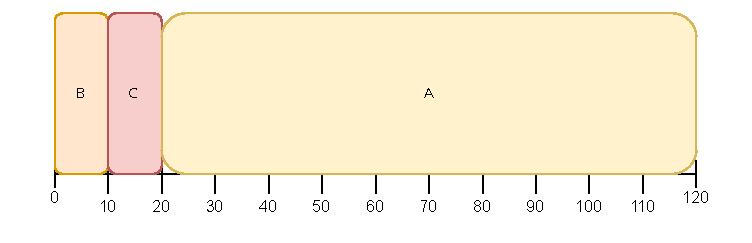
\includegraphics[width=0.9\textwidth]{src/sjf.pdf}
    \caption{Trabajo mas corto primero (SJF)}
\end{figure}

Tomando el mismo ejemplo pero aplicando el algoritmo SJF, el diagrama debería aclarar por qué SJF tiene un rendimiento mucho mejor con respecto al tiempo medio de entrega. Simplemente ejecutando B y C antes que A, SJF reduce el tiempo medio de entrega de 110 segundos a 50 ($\frac{10+20+120}{3}=50$).

\newpage
Ahora supongamos que los procesos no llegan al mismo tiempo: $A$ llega en $t=0$ y necesita ejecutarse durante $100$ segundos, mientras que $B$ y $C$ llegan en $t=10$ y cada uno necesita ejecutarse durante $10$ segundos. Con el algoritmo SJF, el tiempo medio de entrega para los tres trabajos es $\frac{100+(110-10)+(120-10)}{3}=103.33$.
\begin{figure}[h]
    \centering
    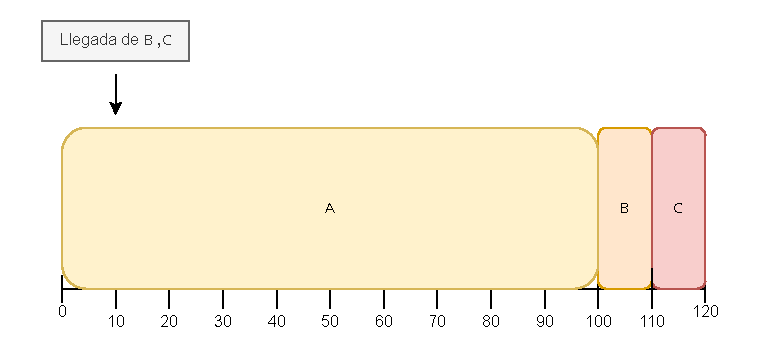
\includegraphics[width=0.9\textwidth]{src/sjf1.pdf}
    \caption{Trabajo mas corto primero (SJF)}
\end{figure}

\subsection{Trabajo de Menor Tiempo Restante Primero (STCF)}
Para solucionar el problema que surgió antes, llega un proceso largo y luego de un rato llegan muchos mas cortos, los cortos tienen un tiempo de espera muy largo cuando podrían ejecutarse antes, en este planificador esto no pasa, ya que cada vez que un nuevo trabajo ingresa al sistema, el planificador STCF determina a cuál de los trabajos restates (incluyendo el nuevo trabajo) le queda el menor tiempo hasta finalizar, y lo elige para ser ejecutado. Por lo tanto, en nuestro ejemplo, STCF habría detenido a A y ejecutado a B y a C hasta su finalización; y recién cuando hayan terminado, habría elegido ejecutar lo que quede de A. 

\begin{figure}[h]
    \centering
    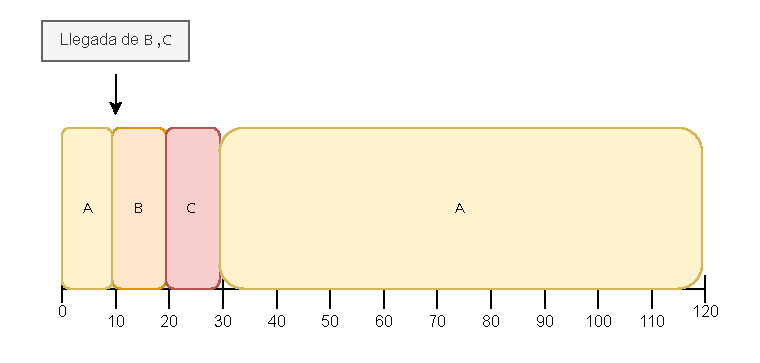
\includegraphics[width=0.9\textwidth]{src/stcf.pdf}
    \caption{Trabajo de Menor Tiempo Restante Primero (STCF)}
\end{figure}

El resultado es un tiempo de entrega mucho mejor (50segs) que el obtenido con SJF (103.33segs). 

\subsection{Round Robin}
Si hablamos de procesos interactivos, es decir aquellos que interactúan constantemente con sus usuarios y, por lo tanto, pasan mucho tiempo esperando pulsaciones de teclas y operaciones de ratón. Cuando se recibe una entrada, el proceso debe despertarse rápidamente, o el usuario percibirá el sistema como poco receptivo. Se introduce un nuevo concepto de tiempo de respuesta:
\begin{definition}
    El tiempo de respuesta se define como el tiempo desde que el trabajo llega a un sistema hasta la primera vez que es elegido para ser ejecutado:
    \begin{equation*}
        T_{\text{respuesta}} = T_{\text{primera ejecución}} - T_{\text{llegada}}
    \end{equation*}
\end{definition}

Entonces, si tres trabajos llegan al mismo tiempo, por ejemplo, el tercer trabajo tiene que esperar a que los dos trabajos anteriores se ejecuten en su totalidad antes de ser elegido por primera vez. Si bien es excelente para el tiempo de entrega, este acercamiento es bastante malo para el tiempo de respuesta y para la interactividad. Es más, imaginate sentado en una terminal, escribiendo, y teniendo que esperar 10 segundos para ver una respuesta del sistema simplemente porque se eligió ejecutar otro trabajo antes que el tuyo. \footnote{OSTEP, Cap.6, Ejecución Directa Limitada}

Acá entra el planificador \textbf{Round Robin}, que es sensible al tiempo de respuesta. La idea básica es simple: en lugar de ejecutar trabajos hasta su finalización, ejecuta cada trabajo durante un segmento de tiempo (a veces llamado quantum de planificación) y luego cambia al siguiente trabajo en la cola de ejecución. Esto lo hace repetidamente hasta que se terminan todos los trabajos. Por esta razón, RR se denomina a veces como división de tiempo. Notemos que la duración de un segmento de tiempo debe ser un múltiplo del período de interrupción del temporizador; por lo tanto, si el temporizador se interrumpe cada 10 milisegundos, el segmento de tiempo podría ser de 10, 20 o cualquier otro múltiplo de 10 ms.

\begin{figure}[h]
    \centering
    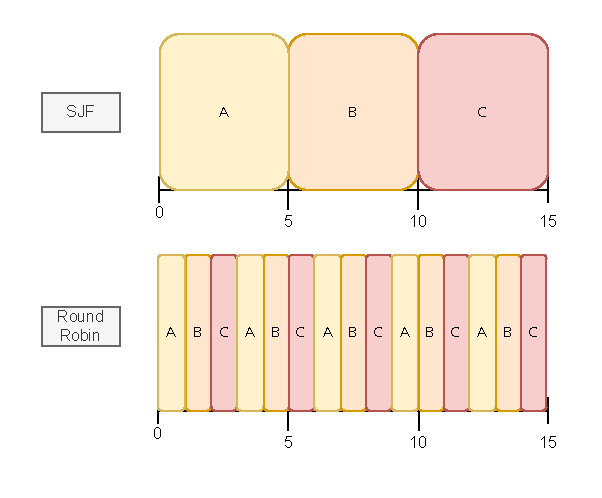
\includegraphics[width=0.9\textwidth]{src/rr.pdf}
    \caption{Round Robin}
\end{figure}

\begin{summary}{Observaciones}
    \begin{itemize}
        \item Cuanto más corto sea el segmento de duración, mejor será el rendimiento de RR según la métrica del tiempo de respuesta. Sin embargo, si el segmento de tiempo es demasiado corto puede resultar problemático: de repente, el costo del cambio de contexto dominaría el rendimiento general. Por lo tanto, decidir la duración del segmento de tiempo presenta un intercambio que el diseñador del sistema debe estar dispuesto a hacer; tiene que ser suficientemente largo como para amortizar el costo del cambio, pero no tan largo como para que el sistema ya no responda.
        \item Generalmente, cualquier política (como RR) que sea justa, es decir, que divida uniformemente la CPU entre los procesos activos en una escala de tiempo pequeña, tendrá un desempeño deficiente en métricas como el tiempo de entrega. De hecho, este trato es inherente: si estás dispuesto a ser injusto, podés ejecutar los trabajos más cortos hasta su finalización, pero a costa del tiempo de respuesta; si, en cambio, valorás la justicia, el tiempo derespuesta se reduce, pero a costa del tiempo de entrega. Este tipo de intercambio es común en los sistemas; no se puede estar en la misa y en la procesión a la vez.
    \end{itemize}
\end{summary}

\subsection{La Cola Multinivel con retroalimentación}
Las ideas básicas detrás de la planificación, y desarrollado dos tipos de acercamientos distintos. El primero ejecuta el trabajo más corto restante y, por lo tanto, optimiza el tiempo de entrega; el segundo alterna entre todos los trabajos y optimiza así el tiempo de respuesta. Por desgracia, ambos son malos donde el otro es bueno, un intercambio inherente que es común en los sistemas.Pero no se resolvió el problema de la incapacidad fundamental del SO para ver el futuro. Ahora se va a produndizar en un planificador que \textit{utiliza el pasado reciente} para predecir el futuro.

El problema fundamental que la MLFQ intenta abordar tiene dos partes. Primero, busca \textbf{optimizar el tiempo de entrega}, que se realiza ejecutando los trabajos más cortos primero; pero el sistema operativo generalmente \textit{no sabe por cuánto tiempo se ejecutará un trabajo}, que es exactamente el conocimiento que requieren los algoritmos como SJF (o STCF). En segundo lugar, MLFQ  quiere \textbf{hacer que el sistema se sienta receptivo a los usuarios interactivos}, y así minimizar el tiempo de respuesta; pero también hay una contra, algoritmos como Round Robin reducen el tiempo de respuesta, pero son terribles para el tiempo de entrega. Entonces, nuestro problema: dado que en general no sabemos nada sobre un proceso, ¿cómo podemos construir un planificador para lograr estos objetivos? ¿Cómo puede el planificador aprender, mientras el sistema se está ejecutando, las características de los trabajos que está corriendo, y así tomar mejores decisiones de planificación? \footnote{OSTEP, Cap.8, MLFQ}

La MLFQ tiene varias \textbf{colas} distintas, a cada una de las cuales se le asigna un nivel de prioridad diferente. En un momento dado, cada trabajo que está listo para ejecutarse se encuentra en una sola cola. MLFQ usa las prioridades para decidir qué trabajo debe ejecutarse en un momento determinado: se elige para ser ejecutado un trabajo con una mayor prioridad (es decir, un trabajo en una cola más alta). Por supuesto, puede haber más de un trabajo en una cola determinada y, por lo tanto, tener la misma prioridad. En este caso, simplemente usaremos planificación round-robin entre estos trabajos.

Con esto surge la pregunta de \textit{¿cómo establece las prioridades?} En lugar de dar una prioridad fija a cada trabajo, MLFQ varía la prioridad de un trabajo en función de su comportamiento observado. Si, por ejemplo, un trabajo renuncia repetidamente a la CPU mientras espera la entrada del teclado, MLFQ mantendrá su prioridad alta, ya que así es como podría comportarse un proceso interactivo. Si, en cambio, un trabajo usa la CPU de manera intensiva durante largos períodos de tiempo, MLFQ reducirá su prioridad. De esta manera, MLFQ intentará aprender sobre los procesos a medida que se ejecutan y, por lo tanto, utilizará el historial del trabajo para predecir su comportamiento futuro.

\subsubsection{Reglas de la MLFQ}
El conjunto de reglas refinadas de la MLFQ son las siguientes:
\begin{enumerate}
    \item Si $\text{Prioridad}(A)>\text{Prioridad}(B)$, se ejecuta A.
    \item Si $\text{Prioridad}(A)=\text{Prioridad}(B)$, se ejecutan en round-robin.
    \item Cuando un trabajo ingresa al sistema,  se coloca en la prioridad más alta (la cola de más arriba).
    \item Una vez que un trabajo utilice su tiempo asignado en un nivel dado (independientemente de cuántas veces haya renunciado a la CPU), su prioridad se reduce (es decir, se mueve una cola hacia abajo).
    \item Después de un período de tiempo determinado S, mover todos los trabajos del sistema a la cola más alta.
\end{enumerate}

\subsubsection{Ejemplos}

En este ejemplo se tienen dos procesos, A en negro, y B en gris, A comienza ejecutandose, al pasar un segmento de tiempo baja y asi hasta llegar a la cola de menor prioridad donde se ejecuta por un tiempo prolongado. Pero en el tiempo $T=100$ llega el proceso B, que comienza también en la cola de mayor prioridad pero con la diferencia de que como esté tiene un tiempo mas corto, al consumir dos segmentos de tiempo ya se terminó de ejecutar, por lo que no llega a estar en menor prioridad. Luego de terminar el proceso A sigue con normalidad.
\begin{figure}[h]
    \centering
    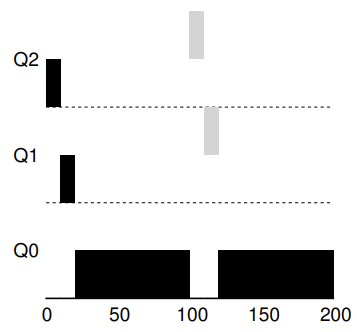
\includegraphics[width=0.4\textwidth]{src/mlfq.png}
    \caption{Cola Multinivel con retroalimentación - Ejemplo 1}
\end{figure}

Ahora supongamos que tenemos un proceso B interactivo, es decir con I/O incluido, sabemos que un proceso abandona la CPU cuando tiene muchas peticiones I/O porque las operaciones de entrada/salida tienden a ser más lentas que las operaciones de procesamiento que se realizan en la CPU. Cuando un proceso realiza una solicitud de I/O, como leer o escribir en un disco, comunicarse con una red o esperar una entrada del usuario, la CPU no puede continuar ejecutando ese proceso hasta que la operación de I/O se complete. Una consecuencia de la \textbf{regla 4}, es que si un proceso abandona el procesador antes de usar un segmento de tiempo, este se mantien en la misma prioridad. Acá podemos ver el objeto de esta regla: \textit{si un trabajo interactivo, por ejemplo, está haciendo una gran cantidad de I/O, abandonará la CPU antes de que se complete su segmento de tiempo; en tal caso, no queremos penalizar el trabajo y, por lo tanto, simplemente lo mantenemos en el mismo nivel.}

\begin{figure}[h]
    \centering
    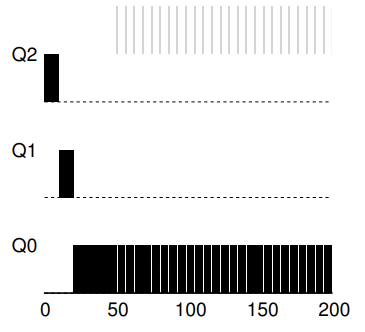
\includegraphics[width=0.4\textwidth]{src/mlfq2.png}
    \caption{Cola Multinivel con retroalimentación - Ejemplo 2}
\end{figure}
\newpage
Un ejemplo para comprender el objetivo de la \textbf{regla 5} es el siguiente, en la izquierda, no hay un impulso de prioridad y, por lo tanto el trabajo de larga duración se muere de hambre una vez que llegan los dos trabajos cortos; en la derecha, hay un impulso de prioridad cada 50 ms (que probablemente sea un valor demasiado pequeño, pero se utiliza aquí para el ejemplo) y, por lo tanto, al menos garantizamos que el trabajo de larga duración progresará, obteniendo un impulso a la máxima prioridad cada 50 ms y así llegar a ejecutarse periódicamente.

\begin{figure}[h]
    \centering
    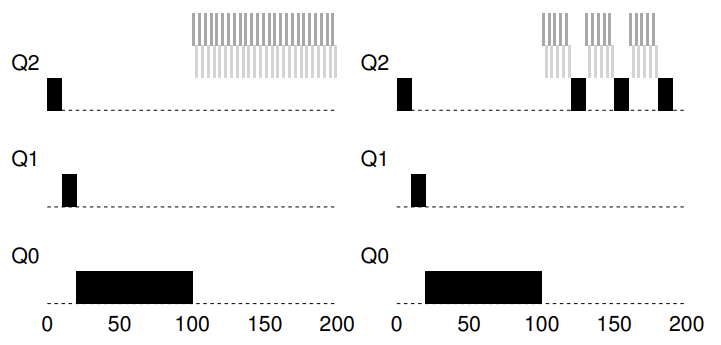
\includegraphics[width=0.8\textwidth]{src/mlfq3.png}
    \caption{Cola Multinivel con retroalimentación - Ejemplo 3}
\end{figure}

Ahora bien, cuando un proceso intenta "engañar" al planificador, con peticiones I/O antes del segmento de tiempo para así mantenerse con mayor prioridad entra la \textbf{regla 4}, una vez que un proceso haya utilizado todo su tiempo asignado, es degradado a la siguiente cola de prioridad. No importa si utiliza el segmento de tiempo en una ráfaga larga o en muchas pequeñas. Así podemos ver en la figura del lado izquierdo no se implementaría esta regla, y el lado derecho si.

\begin{figure}[h]
    \centering
    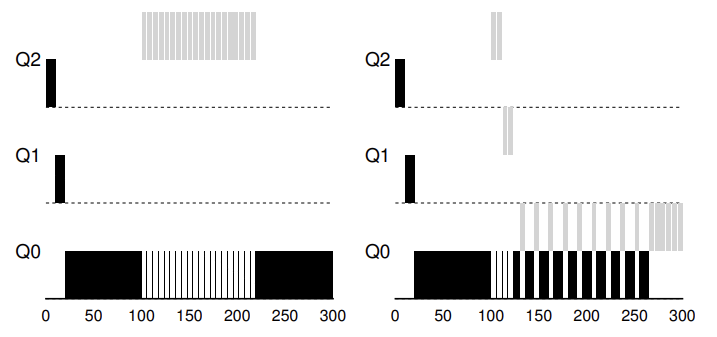
\includegraphics[width=0.8\textwidth]{src/mlfq4.png}
    \caption{Cola Multinivel con retroalimentación - Ejemplo 4}
\end{figure}


\newpage
\section{Espacio de Direcciones}
Llamamos espacio de direcciones a la vista de la memoria del programa en ejecución en el sistema. Este contiene todo el estado de la memoria del programa en ejecución:
\begin{itemize}
    \item El código del programa.
    \item El programa mientras se ejecuta, utiliza una pila (\textbf{stack}) para llevar un registro de donde se encuentra en la cadena de llamadas a funciones, asi como para asignar variables locales y pasar parámetros y valores de retorno entre las rutinas.
    \item También tiene un montículo (\textbf{heap}) que se utiliza para almacenar datos dinámicos, como estructuras de datos que se asignan y liberan en tiempo de ejecución. Lo que se obtiene mediante llamadas a \texttt{malloc()}.
\end{itemize}

\begin{figure}[h]
    \centering
    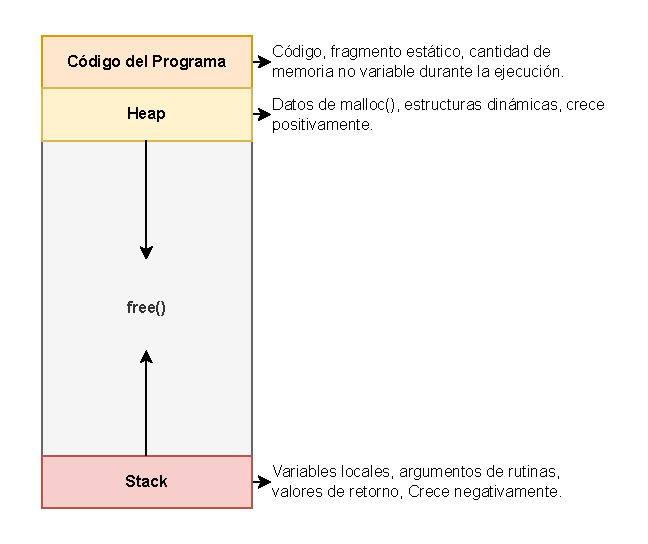
\includegraphics[width=0.62\textwidth]{src/memory.pdf}
    \caption{Stack y Heap}
\end{figure}

El concepto de \textbf{virtualización de memoria} está directamente relacionado con la estructura del espacio de direcciones que describes, ya que esta estructura es una abstracción que el sistema operativo proporciona al programa en ejecución, permitiéndole tener una vista unificada y continua de la memoria, a pesar de que los datos puedan estar físicamente dispersos o no corresponder a los mismos valores de direcciones.

\begin{itemize}
    \item \textbf{Espacio de direcciones virtual}: El código, la pila (stack) y el montículo (heap) existen en el espacio de direcciones virtual, que es lo que el programa percibe como su propio entorno de memoria. Sin embargo, este espacio de direcciones no corresponde directamente a ubicaciones en la memoria física. El sistema operativo y el hardware (a través de la unidad de gestión de memoria o MMU, Memory Management Unit) se encargan de mapear estas direcciones virtuales a direcciones físicas reales.
    \item \textbf{Aislamiento y seguridad}: La virtualización de la memoria permite que múltiples procesos tengan su propio espacio de direcciones virtual, lo que asegura que cada proceso tenga una vista aislada de la memoria, sin interferir con los demás. Por ejemplo, aunque dos procesos distintos tengan una pila o un montículo ubicados en la misma dirección virtual (digamos, ambos comienzan su pila en la dirección 0x1000), sus datos se almacenan en diferentes lugares de la memoria física.
    \item \textbf{Optimización del uso de memoria}: La pila y el montículo en un espacio de direcciones pueden expandirse y contraerse según sea necesario, y el sistema operativo asigna más memoria física o la libera de acuerdo a estas solicitudes. El uso de virtualización de memoria permite que este crecimiento dinámico no esté limitado por la fragmentación o disponibilidad contigua de memoria física, ya que las direcciones virtuales pueden mapearse a bloques de memoria física discontiguos.
    \item \textbf{Manejo de la memoria}: El uso de llamadas como malloc() para asignar memoria en el montículo (heap) o el uso de la pila (stack) para la gestión de llamadas a funciones es completamente manejado en el espacio de direcciones virtual. El programa "piensa" que está operando en direcciones de memoria específicas, pero el sistema operativo se encarga de traducir esas direcciones virtuales en direcciones físicas reales.
\end{itemize}

\subsection{Virtualización de memoria}
Para asegurarse de que el sistema operativo pueda asignar y liberar memoria de manera eficiente, se utiliza la virtualización de memoria. La virtualización de memoria es un mecanismo que permite que un programa en ejecución tenga una vista unificada y continua de la memoria, a pesar de que los datos pueden estar físicamente dispersos o no corresponder a los mismos valores de direcciones. \footnote{OSTEP, Cap.9, Virtualización de Memoria} Hay que tener en cuenta ciertos objetivos:
\begin{enumerate}
    \item Un objetivo principal de un sistema de memoria virtual (VM) es la \textbf{transparencia}. El sistema operativo debe implementar la memoria virtual de una manera que sea invisible para el programa en ejecución. Es decir, el programa no debe ser consciente del hecho de que la memoria está siendo virtualizada; más bien, el programa debe comportarse como si tuviera su propia memoria física privada. Detrás de escena, el sistema operativo (y el hardware) realiza todo el trabajo para multiplexar la memoria entre muchos trabajos diferentes, creando así la ilusión de que cada programa tiene su propia memoria.
    \item Otro objetivo de la memoria virtual es la \textbf{eficiencia}. El sistema operativo debe esforzarse por hacer que la virtualización sea lo más eficiente posible, tanto en términos de tiempo (es decir, sin hacer que los programas se ejecuten mucho más lentamente) como de espacio (es decir, sin usar demasiada memoria para las estructuras necesarias para soportar la virtualización). Para implementar una virtualización eficiente en tiempo, el sistema operativo tendrá que depender del soporte de hardware, incluyendo características de hardware como las TLB (de las que aprenderemos a su debido tiempo).
    \item Un tercer objetivo de la memoria virtual es la \textbf{protección}. El sistema operativo debe asegurarse de proteger los procesos entre sí, así como de protegerse a sí mismo de los procesos. Cuando un proceso realiza una operación de carga, almacenamiento o ejecución de una instrucción, no debe poder acceder ni afectar de ninguna manera el contenido de memoria de ningún otro proceso ni del propio sistema operativo (es decir, nada fuera de su espacio de direcciones). La protección, por lo tanto, nos permite ofrecer la propiedad de aislamiento entre procesos; cada proceso debe ejecutarse en su propio entorno aislado, protegido de los fallos o incluso de los procesos maliciosos.
\end{enumerate}

\newpage
\section{API de Memoria}

\subsection{Tipos de memoria}
\begin{enumerate}
    \item Memoria de la pila \textbf{(Stack memory)}: todas sus asignaciones y liberaciones se gestionan automáticamente. Para declarar algo en la pila en C, simplemente se declara una variable. 
    \begin{verbatim}
    void foo() {
        int x = 42;
    }
    \end{verbatim}
    En este caso, la variable \texttt{x} se asigna en la pila y se libera automáticamente cuando la función \texttt{foo()} termina de ejecutarse. Podría decirse que entonces si queremos un valor que permanezca mas allá de nuestra función, aca entra en juego el \textbf{heap}.
    \item Memoria del montículo \textbf{(Heap memory)}: es un espacio de memoria más grande y más flexible que se puede asignar y liberar manualmente. En C, se utiliza la función \texttt{malloc()} para asignar memoria en el montículo y \texttt{free()} para liberarla.
    \begin{verbatim}
    void foo() {
        int *x = (int *)malloc(sizeof(int));
        ..
    }
    \end{verbatim}
    En este caso, la variable \texttt{x} se asigna en el montículo y no se libera automáticamente cuando la función \texttt{foo()} termina de ejecutarse. Por lo tanto, es responsabilidad del programador liberar la memoria asignada en el montículo cuando ya no se necesite.
\end{enumerate}

\subsection{Llamadas \texttt{malloc()} y \texttt{free()}}
\begin{enumerate}
    \item La llamada \texttt{malloc()} es simplemente decirle que tamaño del espacio que estas solicitando del \textbf{heap} y te devuelve un puntero a la dirección de memoria donde se encuentra ese espacio o \texttt{NULL} si no hay suficiente espacio.
    \begin{verbatim}
    void *malloc(size_t size);
    \end{verbatim}
    El único parámetro que toma \texttt{malloc()} es de tipo \texttt{size\_t}, que simplemente describe cuántos bytes necesitas. Por ejemplo si se quiere reservar memoria para un punto flotante de 8 bytes, se puede hacer de la siguiente manera:
    \begin{verbatim}
    double *x = (double *)malloc(sizeof(double));
    \end{verbatim}
    ¿Cómo está implementada la llamada a \texttt{malloc()}? Voy a introducir una posible implementación sin la certeza de que realmente este hecho de esa forma. 
    \begin{itemize}
        \item \texttt{malloc.c} contiene la estructura \texttt{meta\_block} que almacena información sobre el bloque de memoria.
        \item Cada \texttt{meta\_block} es un nodo en la lista doblemente enlazada. El encabezado de la lista doblemente enlazada se mantiene globalmente en la variable base. Y almacena información como: el \textbf{tamaño del bloque de memoria} correspondiente, \textbf{si el bloque de memoria correspondiente está libre} o no, la \textbf{dirección del nodo siguiente y anterior} en la lista doblemente enlazada, \textbf{puntero al inicio del bloque de memoria} utilizado para almacenar información, una variable de matriz de caracteres que no almacena ningún valor, pero se utiliza para obtener la dirección desde donde se pueden almacenar los datos.
        \item Cuando se invoca, la función \texttt{find\_suitable\_block()} busca si existe un bloque de memoria libre con al menos la cantidad de espacio requerida que esté libre al recorrer la lista vinculada.
        \item Cuando se invoca, la función \texttt{split\_space()} divide el bloque de memoria en dos si contiene suficiente espacio que pueda usarse para almacenar datos.
        \item Cuando se invoca, la función \texttt{extend\_heap()} extiende el montón y agrega un nuevo bloque de memoria a la lista vinculada.
        \item Cuando se llama a la función \texttt{malloc()}:
        \begin{enumerate}
            \item Crea un nuevo bloque invocando \texttt{extend\_heap()} si basees NULL.
            \item De lo contrario, itera a través de la lista enlazada para encontrar si hay algún bloque adecuado (bloque con el tamaño mínimo solicitado).
            \item Si se encuentra un bloque adecuado, se devuelve.
            \item De lo contrario, extiende el montón y devuelve el bloque recién creado.
            \item También verifica si el bloque encontrado en la lista enlazada tiene suficiente espacio extra para ser dividido. En este caso, \texttt{split\_space()} se invoca .
        \end{enumerate}
        El código completo se puede encontrar en \href{https://github.com/RAGUL1902/Dynamic-Memory-Allocation-in-C/blob/master/malloc.c}{este enlace}.

        \item La llamada \texttt{free()} simplemente libera el espacio de memoria asignado previamente por \texttt{malloc()}. Simplemente toma un argumento, el puntero a la memoria retornado por \texttt{malloc()}.
    \end{itemize}
\end{enumerate}

\begin{summary}{Errore comunes}
    \begin{itemize}
        \item Siempre que se declara un puntero para tomar memoria en el montículo, si o sí debe reservarse la memoria antes de usarla.
        \item Si se va a guardar dinámicamente una cadena de caracteres, siempre hay que reservar un byte adicional para el carácter nulo que indica el final de la cadena. Es decir:
        \begin{verbatim}
            char *src = "hello";
            char *dst = (char *)malloc(strlen(src) + 1);
            strcpy(dst, src);
        \end{verbatim}
        \item Si no se reserva la cantidad de memoria correspondiente y se intenta escribir en un espacio de memoria no asignado, se producirá un error de segmentación.
        \item Siempre que se alloca memoria, se debe liberar la memoria una vez que ya no se necesite. Si no se libera la memoria, se produce una fuga de memoria.
        \item Otro error común es el \textbf{double free}, que ocurre cuando se intenta liberar la misma memoria dos veces.
    \end{itemize}
\end{summary}

\section{El mecanismo de traducción de direcciones}
Cuando virtualizabamos la CPU, se buscaba correr el código de un programa directamente en el hardware con la ejecución directa limitada, pero también se necesita virtualizar la memoria. Se va a usar un enfoque similar intentanto lograr tanto \textbf{eficiencia} como \textbf{control} mientras se produce la virtualización. Además de esto, ahora necesitaremos flexibilidad, ya que vamos a necesitar acomodar todos los procesos que se puedan en RAM y que sean fáciles de programar. 
\footnote{OSTEP, Cap.15, Mecanismo de Traducción de Direcciones}
\begin{definition}
    La \textbf{traducción de direcciones}: cada acceso a memoria por \texttt{instruction fetch}, \texttt{load} o \texttt{store} se traduce de memoria virtual, donde el proceso piensa que está accediendo a la memoria, a memoria física, donde realmente se almacenan los datos. La traducción de direcciones es un componente clave de la virtualización de memoria, ya que permite que un programa en ejecución tenga una vista unificada y continua de la memoria, a pesar de que los datos pueden estar físicamente dispersos o no corresponder a los mismos valores de direcciones.
\end{definition}

\textit{Todas y cada una de las referencias a la memoria virtual del proceso que esta corriendo en LDE, tienen que ser traducidas a direcciones reales}. De esto se encarga el hardware, te brinda los mecanismos clave y el sistema operativo los tiene que configurar y usar. Para tomar acciones si un proceso se sale de su espacio y administrar la memoria libre de la computadora. \footnote{Podcast - Nicolas Wolovick cap15}.

\subsection{Ejemplo simple de entendiiento}
Se tiene un programa que simplemente agarra una variable del stack y la incrementa en 3. El programa se compila en código assembler de la siguiente manera:

\begin{figure}[h]
    \centering
    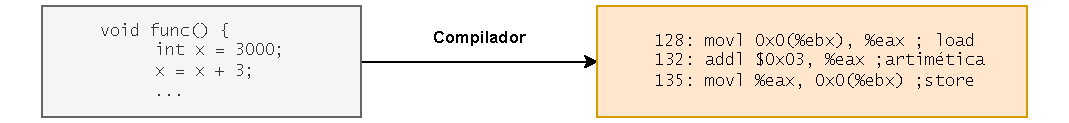
\includegraphics[width=0.8\textwidth]{src/gcc.pdf}
    \caption{Código simple en C y su compilación}
\end{figure}
Ahora supongamos que la variable $x$ se almacena en la dirección $15kb$. La traza de memoria sería la siguiente:
\begin{itemize}
    \item[1.] \texttt{Fetch instruction} en 128.
    \item[2.] \texttt{Load} en 15kb.
    \item[3.] \texttt{Fetch instruction} en 132.
    \item[4.] \texttt{Fetch instruction} en 135.
    \item[5.] \texttt{Store} en 15kb.
\end{itemize}

Desde perspectiva del programa, tiene su espacio de direcciones de una forma y la memoria física se ve diferente:

\begin{figure}[h]
    \centering
    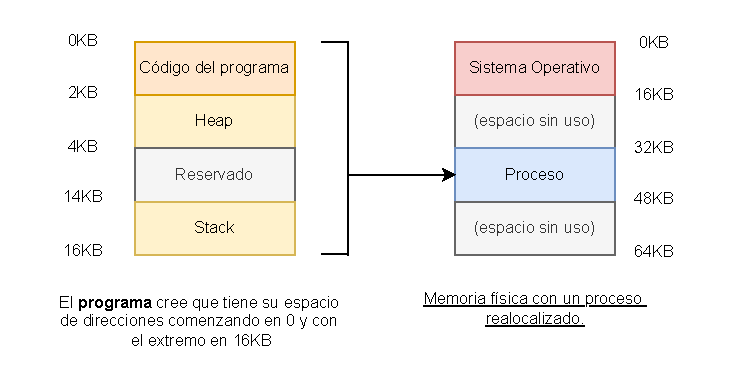
\includegraphics[width=0.8\textwidth]{src/realocatedp.pdf}
    \caption{Traducción de direcciones}
\end{figure}

Este proceso de realocalización es lo que se conoce como \textbf{traducción de direcciones}. El hardware se encarga de realizar esta traducción, y el sistema operativo se encarga de configurar y mantener la tabla de traducción de direcciones.

\subsection{Realocalización dinámica}
Para comprender esta técnica, primero se necesitan dos registros, \textbf{registro base} y \textbf{registro límite}. El registro base contiene la dirección física donde comienza el espacio de direcciones del proceso, y el registro límite contiene el tamaño del espacio de direcciones del proceso. Cuando se realiza una referencia a la memoria, el hardware verifica que la dirección virtual esté dentro del rango permitido por el registro base y el registro límite. Si la dirección virtual está fuera de este rango, se produce un error de segmentación. \footnote{OSTEP, Cap.15, Mecanismo de Traducción de Direcciones}. Con esta configuración, cada programa se escribe y compila como si estuviese cargado en la dirección cero. Sin embargo cuando se ejecuta, el sistema operativo decide donde cargarse en la memoria física y establece el registro base. Por ejemplo en el diagrama anterior el registro base se posiciona en 32KB. Entonces cuando el proceso genere cualquier referencia de memoria se traduce como: \textbf{dirección física = dirección virtual + registro base}. Y el registro límite se establece por el sistema operativo tomando en cuenta el espacio de direcciones, es decir \textbf{registro límite = registro base + tamaño del espacio de direcciones}. El registro límite se revisa en cada acceso a memoria virtual, si se accede por fuera, es decir a posiciones ilegales de la memoria, el hardware genera un trap.

\begin{summary}{Apoyo del hardware}
    \begin{itemize}
        \item Modo protegido: un bit en la \textbf{processor status word}, para que los procesos de usuario no ejecuten operaciones privilegiadas.
        \item Nos brinda los registros \textbf{base and bounds}, base y límite, que permiten la traducción de direcciones de memoria y revisar los límites.
        \item Debe tener ademas \textbf{capacidad de traducción} de virtual a física y revisor de límites. Circuitos que comparan con el límite, y si está en dicho límite, se hace el desplazamiento necesario.
        \item También deben tener \textbf{instrucciones protegidas} que nos permitan cambiar la base y el límite.
        \item \textbf{Instrucciones protegidas} para registrar los administradores de excepciones, el sistema operativo le debe decir al hardware que ejecutar si ocurre algo raro, ya sea una dirección fuera de rango o una instrucción privilegiada.
        \item Finalmente, el hardware debe tener \textbf{capacidad de generar excepciones}, cuando ocurre algo excepcional, el procesador tiene que levantar una excepción.
    \end{itemize}
\end{summary}

\begin{summary}{Combinación de hardware y el sistema operativo}
    El hardware y el sistema operativo cooperan produciendo una implementación de memoria virtual muy sencilla:
    \begin{itemize}
        \item \textbf{Buscar espacio para un proceso nuevo}: teniendo un tamaño fijo, se define una lista enlazada donde se almacenen bloques libres, denominada \textbf{lista de bloques libres}. Cuando un proceso nuevo llega, el sistema operativo busca un bloque libre en la lista y lo asigna al proceso.
        \item \textbf{Proceso se retira de ejecución}: cuando un proceso termina, el sistema operativo libera el bloque de memoria asignado a ese proceso y lo devuelve a la lista de bloques libres.
        \item \textbf{Cambio de contexto}: en el cambio de contexto, el sistema operativo debe actuar, solamente hay un juego de registros base y límite, luego debemos multiplexar en el tiempo, por lo tanto, almacenarlos en el process control block, y al hacer el cambio de contexto cambiar a los nuevos registros base y límite.
        \item \textbf{Definir los handlers de excepción}: definir que se va a hacer cuando ocurra una excepción de fuera de rango, el sistema operativo debe tomar control con una rutina especial y usualmente se retirará al proceso.
    \end{itemize}
\end{summary}

\newpage
\subsection{Ejercicio de realocalización dinámica}
Asumiendo las siguientes características:
\begin{itemize}
    \item Un espacio de direcciones virtuales de 1KB.
    \item Un registro base en 10000.
    \item Un registro límite en 100.
\end{itemize}
\begin{enumerate}
    \item ¿A cúal de las siguientes \textbf{ubicaciones de memoria física} puede acceder legalmente el programa en ejecución?
    \begin{enumerate}
        \item 0
        \item 1000
        \item 10000
        \item 10050
        \item 10100
    \end{enumerate}
    \item ¿A cúal de las siguientes \textbf{direcciones virtuales} puede acceder legalmente el programa en ejecución?
    \begin{enumerate}
        \item 0
        \item 1000
        \item 10000
        \item 10050
        \item 10100
    \end{enumerate}
\end{enumerate}

Primero planteo los datos que tengo:

\begin{figure}[h]
    \centering
    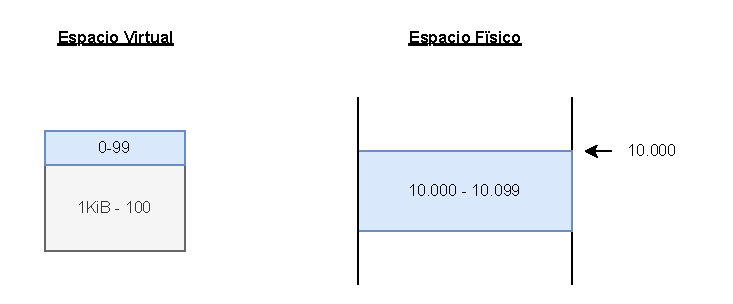
\includegraphics[width=0.5\textwidth]{src/ejtrad.pdf}
    \caption{Datos del ejercicio}
\end{figure}

¿Cómo funcionaría el acceso a memoria dentro de esos límites? El sistema operativo cuando recibe una dirección la compara con el registro límite, y si esa comparación no es exitosa, se lanza la excepción, por lo tanto depende completamente del registro bound.

\begin{figure}[h]
    \centering
    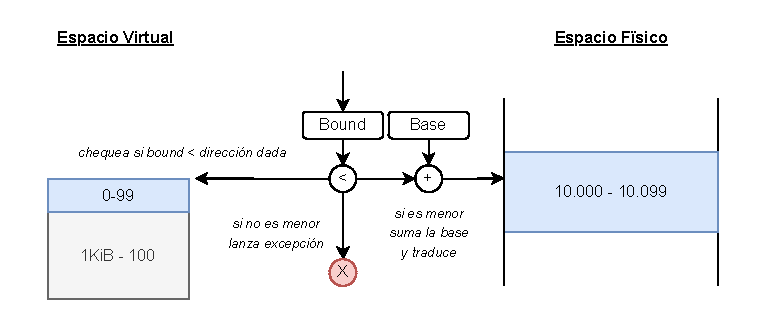
\includegraphics[width=0.8\textwidth]{src/ejtrad2.pdf}
    \caption{Acceso a memoria}
\end{figure}

\newpage
Para el punto 1, sabemos que las direcciones de memoria física a las que se pueden acceder, deben estar dentro del registro bound, entonces, simplemente se debe chequear que queden dentro del rango de direcciones del espacio físico:
\begin{enumerate}
    \item 0 \textbf{No}, ya que está por debajo del registro base.
    \item 1000 \textbf{No}, ya que está por debajo del registro base.
    \item 10000 \textbf{Sí}, ya que está dentro del rango.
    \item 10050 \textbf{Sí}, ya que está dentro del rango.
    \item 10100 \textbf{No}, ya que está en el límite. Los accesos son de 10000 a 10099.
\end{enumerate}
Para el punto 2, es lo mismo, solo que ahora sabemos que el rango de direcciones virtuales es de 0 a 100, entonces:
\begin{enumerate}
    \item 0 \textbf{Sí}, ya que está dentro del rango.
    \item 1000 \textbf{No}, ya que está por encima del límite.
    \item 10000 \textbf{No}, ya que está por encima del límite.
    \item 10050 \textbf{No}, ya que está por encima del límite.
    \item 10100 \textbf{No}, ya que está por encima del límite.
\end{enumerate}

\section{Administración del espacio libre}
\begin{definition}
    Un \textbf{administrador de memoria} es una abstracción que dado un pedazo de mmeoria brinca dos operaciones, \texttt{malloc()} y \texttt{free()}, que permiten pedir y devolver memoria contigua de cualquier tamaño, esta abstracción se usa tanto en espacio de usuario como en espacio del kernel.
\end{definition}
El problema principal de administrar un espacio de memoria contigua donde se piden y devulven pedazos de memoria de longitud variable es la \textbf{fragmentación externa}, es decir, hay espacio libre pero no contiguo. 
\footnote{OSTEP, Cap.17, Administración del Espacio Libre}. 

\subsection{Ejemplo de fragmentación externa}
Supongamos que se produce la siguiente secuencia de eventos:
\begin{enumerate}
    \item Llega el proceso A y pide una cantidad de memoria,
    \item Llega el proceso B y pide el doble de memoria,
    \item LLega el proceso C y pide otra cantidad arbitraria de memoria,
    \item Se bloquea el proceso B,
    \item Llega otro proceso D que se coloca donde estaba el proceso B, pero este ocupa menos por lo que queda otro espacio libre,
    \item Ahora el proceso B se debloquea y pide la misma cantidad de memoria que antes, pero ahora no hay espacio contiguo.
\end{enumerate}

\begin{figure}[h]
    \centering
    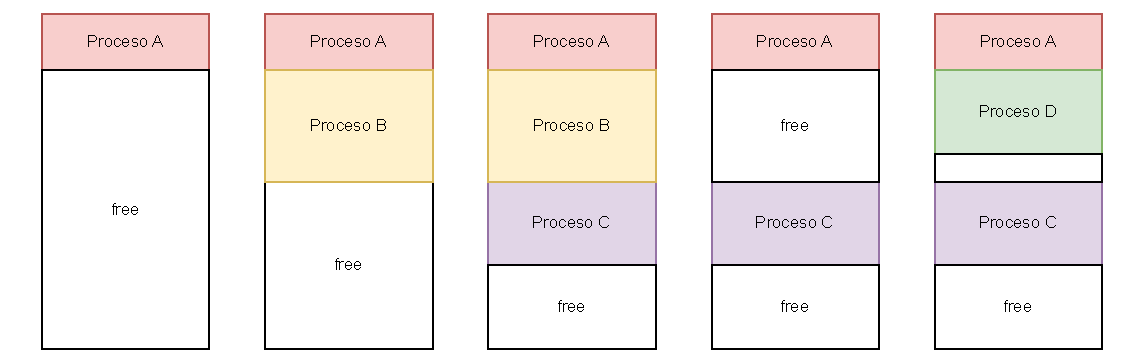
\includegraphics[width=0.9\textwidth]{src/fragexterna.pdf}
    \caption{Fragmentación externa}
\end{figure}

El proceso B no se puede cargar a menos que se saque alguno de los procesos que está cargado en memoria. Es decir estamos aprovechando la memoria de mala manera, se llama fragmentación externa ya que es un problema por fuera de la partición. \footnote{Clase 5 - Hugo Carrer - FCEFyN - UNC}

\subsection{Mecanismo de bajo nivel - División y fusión}
La estructura de datos principal es la \texttt{free list}, que es una lista enlazada de bloques de memoria libres, dados por su dirección en el heap y su longitud. Cuando pedimos memoria de un tamaño $t$, lo que se debe hacer es recorrer los nodos cuyo tamaño sea mayor o igual a $t$ y tomar el primero que se encuentre. Si el tamaño del bloque es mayor que $t$, se divide el bloque en dos, uno de tamaño $t$ y otro de tamaño $s - t$, donde $s$ es el tamaño del bloque original. Si se libera un bloque, se debe recorrer la lista de bloques libres y fusionar los bloques contiguos. 

\begin{definition}
    La fusión, o en inglés \textbf{coalescing}, es el proceso de combinar dos bloques de memoria contiguos en un solo bloque más grande. La fusión es una operación importante en la administración de la memoria, ya que ayuda a reducir la fragmentación externa y a mantener la lista de bloques libres lo más compacta posible.
\end{definition}

Visualmente, supongamos que tenemos el siguiente escenario:
\begin{figure}[h]
    \centering
    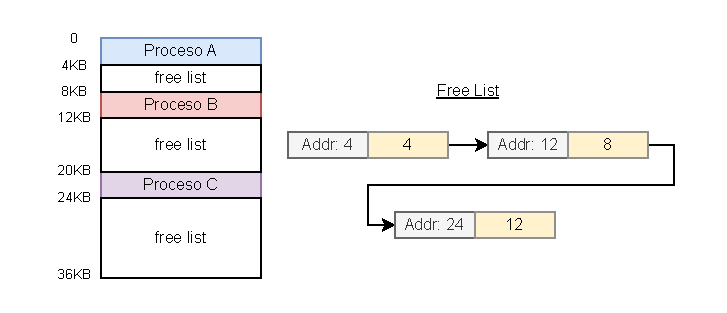
\includegraphics[width=0.9\textwidth]{src/fusion.pdf}
    \caption{Fusión de bloques de memoria}
\end{figure}

Ahora bien, si se libera el Proceso B, que pasa con la free list, podría ya sea alargarse el valor del tamaño del primer nodo hacia adelante, o reducirse la dirección del segundo nodo y alargarse el tamaño también. Acá es donde entra el enfoque de la \textbf{fusión}, donde en vez de modificar uno u otro nodo representante de un segmento libre, los unimos en uno solo.

En el diagrama se mostró una representación visual mas amigable, formalmente podriamos decir que la estructura de la free list en realidad se almacena dentro de dichos espacios libres, de la siguiente manera:

\begin{figure}[h]
    \centering
    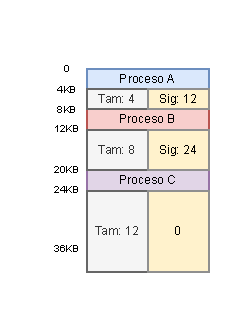
\includegraphics[width=0.3\textwidth]{src/freelist.pdf}
    \caption{Fusión de bloques de memoria - Formal}
\end{figure}

Esto es ya que, como implementariamos una estructura donde se debe usar malloc y free cuando en realidad estamos intentando hacer un manejo de memoria para estos mismos, el famoso problema recursivo de tantos problemas de la computación.

\begin{summary}{Observación}
    Notar que, la llamada \texttt{free(void \*ptr)} no toma un parámetro de tamaño; por lo tanto se asume que, dado un puntero, \texttt{malloc} puede determinar rápidamente el tamaño de la región de memoria que se está liberando y, por ende, reincorporar el espacio a la lista de memoria libre. Para lograr esta tarea, la mayoría de los asignadores almacenan un poco de información adicional en un bloque de encabezado que se mantiene en la memoria, generalmente justo antes del bloque de memoria asignado. 
\end{summary}

Supongamos que se llama a \texttt{ptr = malloc(20)}, el encabezado contiene, como mínimo, el tamaño de la región asignada (en este caso, 20); también puede contener punteros adicionales para acelerar la desasignación, un número mágico para proporcionar verificación de integridad adicional y otra información.

\begin{figure}[h]
    \centering
    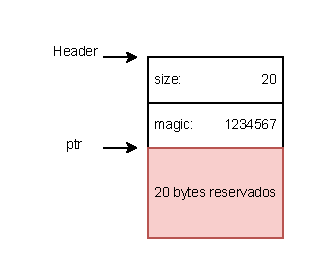
\includegraphics[width=0.5\textwidth]{src/malloc.pdf}
    \caption{Encabezado de un bloque de memoria}
\end{figure}
Entonces se tendría una estructura como esta:
\begin{verbatim}
typedef struct {
    int size;
    int magic;
} header_t;
\end{verbatim}
Cuando el usuario llame a \texttt{free(ptr)}, la biblioteca utiliza aritmética de punteros simple para calcular dónde comienza el encabezado:
\begin{verbatim}
void free(void *ptr) {
    header_t *hptr = (header_t *) ptr - 1;
    ...
}      
\end{verbatim}
Después de obtener dicho puntero al encabezado, la biblioteca puede determinar fácilmente si el número mágico coincide con el valor esperado como una verificación de coherencia (por ejemplo, assert(hptr->magic == 1234567)) y calcular el tamaño total de la región recién liberada mediante matemáticas simples (es decir, sumando el tamaño del encabezado al tamaño de la región). 

\textit{Así se forma una estructura conjunta, en donde se almacena la información necesaria para la administración de la memoria, tanto de los espacios vacíos como de los ocupados. Solucionando el problema de interdependencia.}

\subsection{Políticas de asignación}
Llamamos mecanismo a la forma de lidiar con la estructura de datos, una vez resuelto eso, hay que decidir en cual de todos los lugares posibles vamos a asignar memoria cuando un programa nos pide una cantidad determinada.

\begin{itemize}
    \item \textbf{Best fit}: Elige de entre los espacios libres aquel que tiene la capacidad más parecida al espacio requerido por el nuevo proceso
        \begin{itemize}
            \item Por lo general es el de peor performance.
            \item Lo que garantiza es que el espacio sobrante es el menor posible.
            \item Como consecuencia rápidamente la memoria queda fragmentada en muchos espacios chicos que no pueden albergar un proceso
        \end{itemize}
    \item \textbf{Worst fit}: se asigna el bloque más grande disponible. Esto puede llevar a una fragmentación interna significativa, pero minimiza la fragmentación externa.
    \item \textbf{First fit}: Elige el primer espacio de memoria libre donde entre el proceso nuevo a cargar:
    \begin{itemize}
        \item Es el más simple y rápido.
        \item En muchas condiciones es el mejor.
        \item Genera fragmentación al comienzo de la memoria lo que hace un poco mas lentas las búsquedas subsecuentes.
    \end{itemize}
    \item \textbf{Next fit}: Elige el primer espacio de memoria libre donde entre el proceso nuevo a cargar pero buscando desde la posición donde se cargó el último proceso.
    \begin{itemize}
        \item En este caso se genera fragmentación hacia el final de la memoria.
        \item En general requiere mas frecuencia de compactación que el first-fit.  
    \end{itemize} \footnote{Clase 5 - Hugo Carrer - FCEFyN - UNC}
\end{itemize}

\section{Paginación}
Se dice que el sistema operativo toma uno de dos enfoques al resolver casi cualquier problema de gestión de espacio. El primer enfoque es dividir el espacio en piezas de tamaño variable, llamada \textbf{segmentación en memoria virtual}. Desafortunadamente, esta solución tiene dificultades inherentes. En particular, al dividir un espacio en fragmentos de diferentes tamaños, el espacio en sí puede fragmentarse, lo que hace que la asignación sea más complicada con el tiempo. Por lo tanto, puede valer la pena considerar el segundo enfoque: dividir el espacio en piezas de tamaño fijo. En memoria virtual, llamamos a esta idea \textbf{paginación}. La paginación, como veremos, tiene varias ventajas sobre nuestros enfoques anteriores. Probablemente, la mejora más importante será la flexibilidad: con un enfoque de paginación completamente desarrollado, el sistema podrá soportar la abstracción de un espacio de direcciones de manera efectiva, independientemente de cómo un proceso use el espacio de direcciones. 

\begin{definition}
    La \textbf{paginación} se desarrolla para reducir la fragmentación tanto interna como externa. Consiste en dividir la memoria principal en pedazos de la misma capacidad, relativamente chica, estos pedazos se llaman \textbf{marcos}. Se hace lo mismo con los procesos dividiéndolos en pedazos todos de la misma capacidad de los marcos, estos se conocen como \textbf{páginas}.
\end{definition}

Al momento de cargar el proceso en memoria se asignan las páginas del mismo a un conjunto de marcos libres, no necesariamente contiguos.

Para ilustrar esto, supongamos que se tiene un pequeño espacio de direcciones, con solo 64 bytes en total, con cuatro páginas de 16 bytes (páginas virtuales 0, 1, 2 y 3). La memoria física, también consiste en un número de ranuras de tamaño fijo, en este caso ocho marcos de página. Se puede notar que las páginas del espacio de direcciones virtuales se han colocado en diferentes ubicaciones a lo largo de la memoria física; el diagrama también muestra que el sistema operativo usa parte de la memoria física para sí mismo. 

\begin{figure}[h]
    \centering
    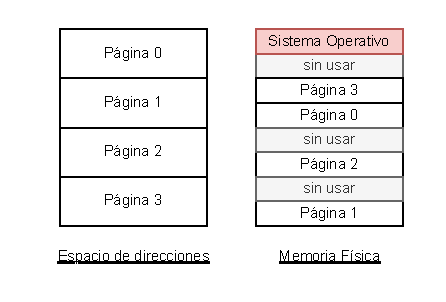
\includegraphics[width=0.6\textwidth]{src/paginacion.pdf}
    \caption{Ejemplo - Paginación}
\end{figure}

Para registrar dónde se coloca cada página virtual del espacio de direcciones en la memoria física, el sistema operativo generalmente mantiene una estructura de datos por proceso conocida como \textbf{tabla de páginas}. El papel principal de la tabla de páginas es almacenar las \textbf{traducciones de direcciones} para cada una de las páginas virtuales del espacio de direcciones, permitiéndonos saber dónde reside cada página en la memoria física. 

En el programa cada dirección se representa como un número de página sumado a un desplazamiento dentro de la página, el número de página se representa como \textbf{VPN} (virtual page number) y el desplazamiento como \textbf{offset}.

\subsection{Ejemplo de traducción de dirección}
Supongamos que el proceso con el espacio de direcciones virtual de la figura anterior esta haciendo un acceso a memoria:
\begin{verbatim}
movl <virtual address>, %eax
\end{verbatim}
Para traducir esta direccion virtual que genero el proceso, primero debemos dividirla en los dos componentes, VPN y offset. Como en este ejemplo el espacio de direcciones es de 64 bytes, necesitariamos 6 bits para la dirección virtual.
\begin{equation*}
    \begin{array}{|c|c|c|c|c|c|}
        \hline
        Va5 & Va4 & Va3 & Va2 & Va1 & Va0 \\
        \hline
    \end{array}
\end{equation*}
Donde Va5 sería el bit mas significativo, y Va0 el de menor orden, como sabemos que la página es de 16 bytes, deberiamos poder asignar 4 páginas, los dos primeros bits se encargan de eso. Ahora bien se quiere cargar la dirección virtual 21, es decir
\begin{verbatim}
movl 21, %eax
\end{verbatim}
Se puede expresar como 010101 en binario, es decir está en el quinto byte de la página 1:
\begin{equation*}
    \begin{array}{|c|c|c|c|c|c|}
        \hline
        Va5 & Va4 & Va3 & Va2 & Va1 & Va0 \\
        \hline
        0 & 1 & 0 & 1 & 0 & 1 \\
        \hline
    \end{array}
\end{equation*}
Ahora con el VPN y el offset, podemos, mediante PFN (physical frame number) y el offset, traducir la dirección virtual a la dirección física. En este caso, la VPN es 0101, es decir la página 1, y el offset es 0101, es decir el quinto byte de la página. La tabla de páginas nos dice que la página 1 se encuentra en el marco físico 7.

\begin{figure}[h]
    \centering
    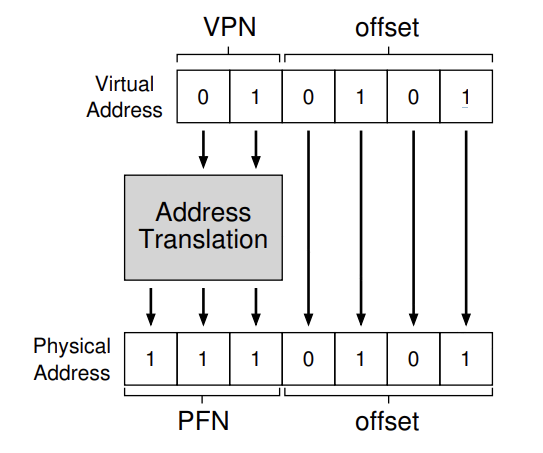
\includegraphics[width=0.5\textwidth]{src/traduccion.png}
    \caption{Traducción de dirección}
\end{figure}

Notar que el desplazamiento sigue igual, esto es ya que el desplazamiento solamente nos indica que byte dentro de la página queremos. La tabla de páginas se guardará en el sistema operativo de la siguiente manera:

\begin{figure}[h]
    \centering
    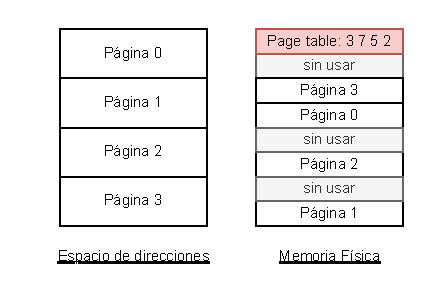
\includegraphics[width=0.6\textwidth]{src/tablapaginas.pdf}
    \caption{Tabla de páginas}
\end{figure}

\subsection{Tabla de páginas}

\begin{definition}
    La tabla de páginas es simplemente una estructura de datos que se utiliza para mapear direcciones virtuales (o realmente, números de páginas virtuales) a direcciones físicas (números de marcos físicos).
\end{definition}

La forma más simple se llama tabla de páginas lineal, que es solo un arreglo. El sistema operativo indexa el arreglo usando el número de página virtual (VPN) y busca la entrada de la tabla de páginas (PTE) en ese índice para encontrar el número de marco físico (PFN) deseado. Consta de lo siguiente:

\begin{itemize}
    \item Un \textbf{bit de validez} es común para indicar si una traducción en particular es válida; por ejemplo, cuando un programa comienza a ejecutarse, tendrá código y un montón en un extremo de su espacio de direcciones, y la pila en el otro. Todo el espacio no utilizado en el medio será marcado como inválido, y si el proceso intenta acceder a esa memoria, generará una excepción al sistema operativo, que probablemente terminará el proceso. Por lo tanto, el bit de validez es crucial para soportar un espacio de direcciones disperso; simplemente marcando todas las páginas no utilizadas como inválidas, eliminamos la necesidad de asignar marcos físicos para esas páginas y, por lo tanto, ahorramos mucha memoria.
    \item[\textbf{PFN}] El número de marco físico (PFN) es el número de marco físico en el que se encuentra la página virtual correspondiente.
    \item[\textbf{R/W}] \textbf{Bits de protección}, que indican si se puede leer, escribir o ejecutar desde la página. == 1 si se puede leer y escribir, == 0 solo lectura.
    \item[\textbf{P}] Un \textbf{bit de presencia} indica si esta página está en la memoria física o en el disco. == 1 la página está en memoria física, == 0 la página no está cargada, la CPU genera una excepción de fallo de página.
    \item[\textbf{D}] Un \textbf{bit de modificación} es también común, indicando si la página ha sido modificada desde que se trajo a la memoria.
    \begin{itemize}
        \item D = 1: se ha escrito en la página, y cuando se necesite eliminarla de la memoria principal será preciso previamente actualizarla en la memoria virtual.
        \item D = 0: se puede sobrescribir cuando se necesita sustituirla por otra ya que no ha sido modificada durante su permanencia en la memoria principal.
    \end{itemize}
    \item[\textbf{A}] Un \textbf{bit de referencia} (también conocido como bit de acceso) se usa a veces para rastrear si una página ha sido accedida, y es útil para determinar qué páginas son populares y, por lo tanto, deberían mantenerse en la memoria. Se pone a 1 cada vez que se accede a dicha p´agina. En un lapso de tiempo, el SO lee este bit, si vale ”1” lo pasa a ”0” e incrementa el contador que tiene asociado a la página, al que le aplica el algoritmo LRU para eliminar de la memoria la página menos usada recientemente.
    \item[\textbf{PCD}] (Aceptación de la Caché): indica si la página se puede o no meter en la memoria Caché.
    \item[\textbf{PWT}] (Escritura obligada): Indica que la página, además de ser cacheable funcion en modo de escritura obligada.
\end{itemize} \footnote{Mag. Ing. Miguel Solinas - Sistemas de Computación - FCEFyN - UNC}

\begin{figure}[h]
    \centering
    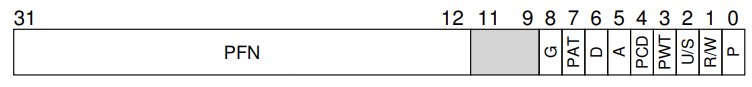
\includegraphics[width=0.8\textwidth]{src/pte.png}
    \caption{Entrada de la tabla de páginas}
\end{figure}

\subsection{Ejemplo completo}
Volviendo al ejemplo anterior, se tiene la siguiente instrucción que se quiere ejecutar:
\begin{verbatim}
movl 21, %eax
\end{verbatim}
El sistema debe traducir la dirección 21 a 117, entonces, \textit{antes de obtener los datos de la dirección 117, el sistema primero debe obtener la entrada de la tabla de páginas correcta del proceso, realizar la traducción y luego cargar los datos desde la memoria física.} Pero para hacer esto, el hardware debe saber dónde está la tabla de páginas del proceso que se está ejecutando. Supongamos por ahora que un solo registro base de la tabla de páginas contiene la dirección física de la ubicación inicial de la tabla de páginas. Para encontrar la ubicación de la PTE deseada, el hardware realizará las siguientes funciones:
\begin{verbatim}
    VPN = (VirtualAddress & VPN_MASK) >> SHIFT
    PTEAddr = PageTableBaseRegister + (VPN * sizeof(PTE))    
\end{verbatim}
En este ejemplo, \texttt{VPN\_MASK} es un número que se usa para enmascarar los bits de la dirección virtual que no son el número de página virtual, y \texttt{SHIFT} es el número de bits que se deben desplazar a la derecha para obtener el número de página virtual. En este caso, VPN\_MASK sería 0x30 y SHIFT sería 4.

Por ejemplo, con la dirección virtual 21 (010101), al aplicar la mascara obtenemos 010000, que es el número de página virtual 1. Luego, se usa este número como índice en el arreglo de PTE's apuntado por el registro base de la tabla de páginas.

Una vez que se conoce esta dirección física, el hardware puede obtener la PTE de la memoria, extraer el PFN, y concatenarlo con el desplazamiento de la dirección virtual para formar la dirección física deseada. Podemos decir que el PFN se desplaza hacia la izquierda por SHIFT, y luego se combina con el desplazamiento mediante una operación OR bit a bit para formar la dirección final de la siguiente manera:
\begin{verbatim}
    offset = VirtualAddress & OFFSET_MASK
    PhysAddr = (PFN << SHIFT) | offset    
\end{verbatim}

Con esto el hardware ya puede obtener los datos de la dirección 117 y cargarlos en el registro \texttt{\%eax}. Entonces, el enfoque completo del manejo de cada referencia de memoria sería algo como:

\begin{verbatim}
    // Extract the VPN from the virtual address
    VPN = (VirtualAddress & VPN_MASK) >> SHIFT
    
    // Form the address of the page-table entry (PTE)
    PTEAddr = PTBR + (VPN * sizeof(PTE))
    
    // Fetch the PTE
    PTE = AccessMemory(PTEAddr)
    
    // Check if process can access the page
    if (PTE.Valid == False)
        RaiseException(SEGMENTATION_FAULT)
    else if (CanAccess(PTE.ProtectBits) == False)
        RaiseException(PROTECTION_FAULT)
    else
    // Access OK: form physical address and fetch it
    offset = VirtualAddress & OFFSET_MASK
    PhysAddr = (PTE.PFN << PFN_SHIFT) | offset
    Register = AccessMemory(PhysAddr)     
\end{verbatim}

Pero con esto surge un problema, sin un diseño cuidadoso tanto del hardware como del software, las tablas de páginas \textbf{harán que el sistema funcione demasiado lento} y ocupen demasiada memoria. 

\subsection{Traza de memoria}
Ahora analizo la cantidad de accesos a memoria que se realizan en el método de paginación. Nos interesa el siguiente fragmento de código:

\begin{verbatim}
    int array[1000];
    ...
    for (i = 0; i < 1000; i++)
        array[i] = 0;    
\end{verbatim}
El código ensamblador que escupe el compilador es:

\begin{verbatim}
1024 movl $0x0,(%edi,%eax,4) ; mueve el 0 a la dirección de memoria a array[i]
1028 incl %eax               ; incrementa el contador
1032 cmpl $0x03e8,%eax       ; compara el contador con 1000
1036 jne 1024                ; si no es igual, salta a 1024
\end{verbatim}

Asumamos que el espacio de direcciones virtual es de 64KB y un tamaño de página de 1KB. Lo único que necesitamos saber ahora es el contenido de la tabla de páginas y su ubicación en la memoria física. Supongamos que tenemos una tabla de páginas lineal (basada en un array) y que se encuentra en la dirección física 1KB (1024).
\begin{itemize}
    \item Primero, está la página virtual donde reside el código. Como el tamaño de página es de 1KB, la dirección virtual 1024 reside en la segunda página del espacio de direcciones virtuales (VPN=1, ya que VPN=0 es la primera página). Supongamos que esta página virtual se mapea al marco físico 4 (VPN 1 $\rightarrow$ PFN 4).
    \item Luego, está el arreglo en sí. Su tamaño es de 4000 bytes (1000 enteros), y asumimos que reside en las direcciones virtuales 40000 a 44000 (sin incluir el último byte). Las páginas virtuales para este rango decimal son VPN=39 ... VPN=42. Por lo tanto, necesitamos mapeos para estas páginas. Supongamos los siguientes mapeos virtual-físicos para el ejemplo: (VPN 39 → PFN 7), (VPN 40 → PFN 8), (VPN 41 → PFN 9), (VPN 42 $\rightarrow$ PFN 10).
\end{itemize}

Cuando se ejecuta, cada búsqueda de instrucción generará dos referencias a la memoria: una a la tabla de páginas para encontrar el marco físico en el que reside la instrucción y otra a la instrucción misma para traerla a la CPU para su procesamiento. Además, hay una referencia explícita a la memoria en forma de la instrucción mov; esto añade otro acceso a la tabla de páginas primero (para traducir la dirección virtual del arreglo a la física correcta) y luego el acceso al arreglo en sí.

\begin{figure}[h]
    \centering
    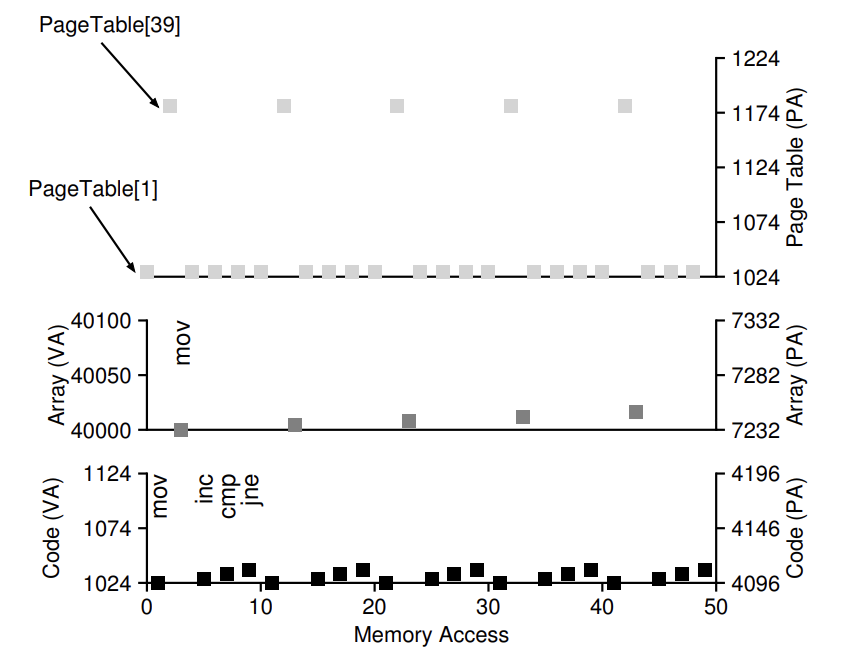
\includegraphics[width=0.8\textwidth]{src/trazamemoria.png}
    \caption{Traza de memoria}
\end{figure}

El gráfico inferior muestra las referencias de memoria de las instrucciones en el eje y en negro (con direcciones virtuales a la izquierda y las direcciones físicas reales a la derecha); el gráfico medio muestra los accesos al arreglo en gris oscuro (nuevamente con virtual a la izquierda y físico a la derecha); finalmente, el gráfico superior muestra los accesos a la tabla de páginas en gris claro (solo físico, ya que la tabla de páginas en este ejemplo reside en memoria física). El eje x, para todo el rastreo, muestra las referencias de memoria a lo largo de las primeras cinco iteraciones del bucle; hay 10 accesos a la memoria por iteración del bucle, que incluyen cuatro búsquedas de instrucciones, una actualización explícita de la memoria, y cinco accesos a la tabla de páginas para traducir esas cuatro búsquedas y una actualización explícita.

\section{TLBs}
La paginación como vimos cada instruction fetch, cada load y cada store, antes deben pasar por la tabla de traducción de marco virtual a marco físico. Para acelerar el proceso de traudcción, el hardware nos brinca una ayuda, introdujo dentro del propio chip una pequeña memoria caché especial ultra rápida, denominada \textbf{Translation Lookaside Buffer} (TLB). Es decir es solamente una caché de traducción.

\subsection{Algoritmo básico de la TLB}
Supongamos que tenemos una tabla de páginas lineal, tendríamos esta secuencia de trabajo:
\begin{enumerate}
    \item Obtener el \textbf{VPN},
    \item Buscar en la TLB, si es un \textbf{hit}, obtenemos el \textbf{PFN} y el \textbf{offset}, si hay un \textbf{miss}, se busca en la tabla de páginas, la PTE que corresponda a esa VPN, se extraen los 20bits de la PFN, se actualiza la TLB con la nueva entrada y se reejecuta la instrucción para que funcione.
\end{enumerate}
Lo que buscamos es aumentar la probabilidad de que la traducción de una dirección virtual a una dirección física se encuentre en la TLB.

\subsection{Ejemplo}
Supongamos que tenemos un arreglo de 10 enteros de 4-bytes en memoria. Se tendría un esquema de memoria virtual de 4 VPN, esto quiere decir que vamos a tener los 4 bits mas significativos de la dirección virtual para la VPN, y los otros 4 para el offset. Cada página tiene 4 enteros. Y vamos a tener A[0] esta en la segunda casilla del marco virtual número 6, entonces
\begin{itemize}
    \item 3 en el marco virtual 6,
    \item 4 en el marco virtual 7,
    \item los 3 finales en el marco virtual 8.
\end{itemize}
Vamos a pensar en este fragmento de código que recorre cada uno de esos elementos en el arreglo y los acumula en un registro del procesador que va a ser la suma de ellos:
\begin{verbatim}
int i, sum = 0;
for (i = 0; i < 10; i++) {
    sum += a[i];
}    
\end{verbatim}
La secuencia va a ser la siguiente:
\begin{enumerate}
    \item Se accede a a[0], el número de página virtual es el 6, que no esta en la TLB, se produce un miss, se busca en la tabla de páginas, se actualiza la TLB y se ejecuta la instrucción.
    \item Vuelve a acceder a a[0] pero esta vez ya está en la TLB, por lo que se produce un hit, se obtiene el PFN y el offset, y se ejecuta la instrucción.
    \item Se accede a a[1], el número de página virtual es el 6, que ya está en la TLB, por lo que se produce un hit, se obtiene el PFN y el offset, y se ejecuta la instrucción.
    \item Se accede a a[2], sigo estando en el marco virtual 6, por lo que se produce un hit, se obtiene el PFN y el offset, y se ejecuta la instrucción.
    \item Se accede a a[3], el número de marco virtual es el 7, que no está en la TLB, por lo que se produce un miss, se busca en la tabla de páginas, se actualiza la TLB y se ejecuta la instrucción.
    \item Se accede a a[4], el número de marco virtual es el 7, que ya está en la TLB, por lo que se produce un hit, se obtiene el PFN y el offset, y se ejecuta la instrucción.
    \item Se accede a a[5], el número de marco virtual es el 7, que ya está en la TLB, por lo que se produce un hit, se obtiene el PFN y el offset, y se ejecuta la instrucción.
    \item Se accede a a[6], el número de marco virtual es el 7, que ya está en la TLB, por lo que se produce un hit, se obtiene el PFN y el offset, y se ejecuta la instrucción.
    \item Se accede a a[7], no está en la TLB, se produce un miss, se busca en la tabla de páginas, se actualiza la TLB y se ejecuta la instrucción.
    \item Se accede a a[8], el número de marco virtual es el 8, que no está en la TLB, se produce un miss, se busca en la tabla de páginas, se actualiza la TLB y se ejecuta la instrucción.
    \item Se accede a a[9], el número de marco virtual es el 8, que ya está en la TLB, por lo que se produce un hit, se obtiene el PFN y el offset, y se ejecuta la instrucción.
\end{enumerate}
De los 10 accesos que hice a la memoria \textbf{7} son TLB hits, y \textbf{3} son TLB misses. 

\begin{summary}{Obervación}
    Notar que el tamaño de página juega un rol muy importante, si el tamaño de página fuese mas grande, producirá menos TLB misses, pero si el tamaño de página es muy grande, se producirá más fragmentación interna. Normalmente el tamaño de página es de 4KB.
\end{summary}

\subsection{TLB miss}

¿Quién administra los TLB miss? En intel x86, el hardware se encarga de esto, esto implica que sabe donde está la page table, esto se logra a través de un registro llamado \textbf{CR3}, tiene que caminar dicha page table hasta encontrar la PTE que corresponde, y luego actualizar la TLB, para luego reintentar la ejecución. 

\begin{definition}
    Un TLB \textbf{miss} es un trap, una excepción, se pasa a kernel mode, se pasa de trap handler, se recorre la page table por software y se obtiene el PFN, se actualiza la TLB mediante una instrucción privilegiada y se hace return from trap.
\end{definition}

\subsection{Estructura y funcionamiento de la TLB}
Una TLB es chica, tiene pocas entradas que asocian un marco virtual a un marco físico, es decir, una VPN a un PFN, este cache se llama completamente asociativo, ya que dado un VPN se consultan las entradas en forma paralela.

Una entrada del TLB debe contener \textbf{VPN}, \textbf{PFN}, y mas información como por ejemplo si la page table está presente o si es válida, además puede contener los bits R/W. Y también contienen un bit que indica si esa entrada de la TLB es válida. 

Notar que al producirse un cambio de contexto, debo poner todos los bits de la TLB en 0, ya que no se puede garantizar que la información que está en la TLB sea válida.

\subsubsection{Cambio de contexto}
Ahora bien, ¿qué pasa cuando se produce un cambio de contexto? Cuando cambiamos de contexto, apuntamos a otra page table, esto implica que todas las entradas de la TLB quedan inválidas, no hay que usar traducciones de virtuales a físicas de otros procesos, es un problema típico de consistencia de caché. 

Supongamos que tenemos el proceso P1 corriendo, y mapea de página virtual a física 10 a 100, cambia de contexto al proceso P2 y el mismo mapea la página virtual 10 en página física 170. ¿Cuál va a ser el contenido de la TLB para la página virtual número 10? La solución simple es tirar la cadena de la TLB en cada cambio de contexto. 

Una solución a esto es agregar un campo llamado \textbf{ASID} (Address Space Identifier) a la TLB, que es un número que identifica a cada proceso, entonces cuando se produce un cambio de contexto, se cambia el ASID, y se puede saber si la entrada de la TLB es válida o no. Así la TLB del proceso se vería como:

\begin{equation*}
    \begin{array}{c|c|c|c|c}
        VPN & PFN & Valid & R/W & ASID \\
        \hline
        10 & 100 & 1 & rwx & 1 \\
        - & - & 0 & - & - \\
        \hline
        10 & 170 & 1 & rwx & 2 \\
        - & - & 0 & - & - \\
    \end{array}
\end{equation*}

\subsection{Políticas de reemplazo de la TLB}
Todo caché tiene un problema, se llena rapidamente, si se llena la TLB y viene una nueva página para traducir de virtual a física, ¿qué entrada tengo que usar para poner la nueva?, esto se denomina \textbf{política de reemplazo}. Si la política de reemplazo es \textbf{LRU} (Least Recently Used), se reemplaza la entrada que no se usó hace más tiempo. Tambíen son válidas las políticas aleatorias, es decir se elige una entrada al azar.

\section{Paginación Multinivel}
Las page table lineales son grandes, por ejemplo en un esquema 20 12, con páginas de 4KB, y 32 bits de espacio de direcciones, la page table lineal ocupa 4Bytes por $2^{20}$ entradas, es decir 4MB. Esto es un problema, ya que si tengo un proceso que solo usa 1MB de memoria, tengo que tener 4MB de page table. Y si tenemos 100 procesos, necesitamos 400MB de page table, lo cual es un problema de sobrecarga. El enfoque de paginación es flexible pero caro.

La solución es simple, páginas mas grandes, al agrandar el tamaño de página, pero si las páginas son grandes, se desperdicia lugar, el famoso problema de fragmentación interna. La mayoria de los sistemas operativos usan páginas chicas. 

\subsection{Solución híbrida}
Se basa en combinar la paginación y la segmentación para reducir la sobrecarga de memoria de las tablas de páginas. Vamos a ver un ejemplo para analizar porqué esto podría funcionar:

Supongamos que tenemos un espacio de direcciones en el que las partes usadas del heap y la pila son pequeñas. Para el ejemplo, usamos un espacio de direcciones de 16KB con páginas de 1KB. 
\begin{figure}[h]
    \centering
    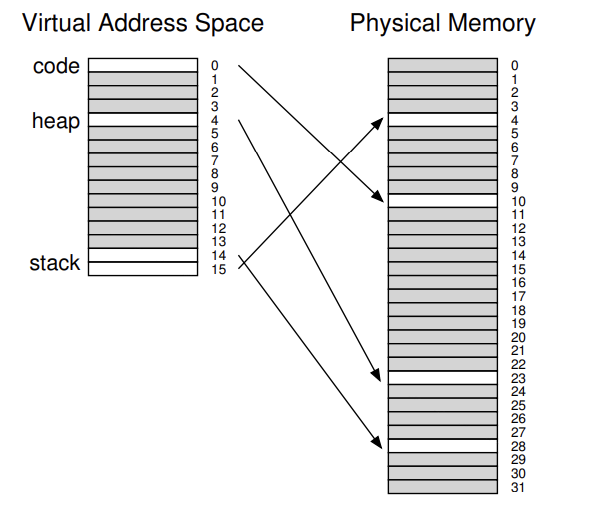
\includegraphics[width=0.6\textwidth]{src/espaciodirecciones.png}
    \caption{Espacio de direcciones - Ejemplo}
\end{figure}
La tabla de páginas para este espacio de direcciones se muestra en la figura siguiente:
\begin{figure}[h]
    \centering
    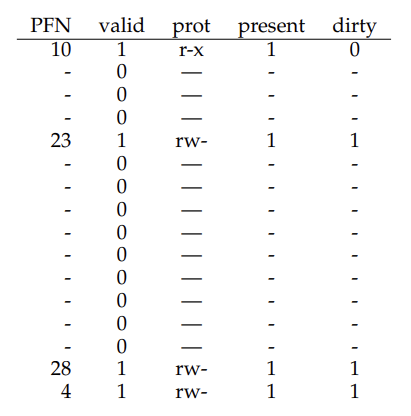
\includegraphics[width=0.4\textwidth]{src/tabla.png}
    \caption{Tabla de páginas - Ejemplo}
\end{figure}
Este ejemplo asume que la única página de código (VPN 0) está asignada a la página física 10, la única página del heap (VPN 4) a la página física 23, y las dos páginas de la pila al otro extremo del espacio de direcciones (VPNs 14 y 15) están asignadas a las páginas físicas 28 y 4, respectivamente. Notar que la mayor parte de la tabla de páginas está sin usar, llena de entradas inválidas.

En nuestro enfoque híbrido, en lugar de tener una sola tabla de páginas para todo el espacio de direcciones del proceso, ¿por qué no tener una por cada segmento lógico? En este ejemplo, podríamos tener tres tablas de páginas, una para el código, el heap y la pila.
\newpage
Para determinar a qué segmento se refiere una dirección, usaremos los dos bits superiores del espacio de direcciones. Supongamos que 00 es el segmento no usado, 01 para el código, 10 para el heap y 11 para la pila. Así, una dirección virtual se ve como esto:
\begin{figure}[h]
    \centering
    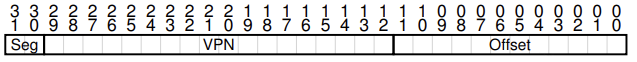
\includegraphics[width=0.7\textwidth]{src/direccion.png}
    \caption{Dirección virtual - Ejemplo}
\end{figure}
En el hardware, supongamos que hay tres pares de registros base/límite, uno para cada código, heap y pila. Cuando un proceso se está ejecutando, el registro base para cada uno de estos segmentos contiene la dirección física de una tabla de páginas lineal para ese segmento; por lo tanto, cada proceso en el sistema ahora tiene tres tablas de páginas asociadas. En un cambio de contexto, estos registros deben cambiarse para reflejar la ubicación de las tablas de páginas del nuevo proceso en ejecución.

En una falta de TLB (asumiendo una TLB gestionada por hardware), el hardware usa los bits del segmento (SN) para determinar qué par de registros base y límite usar. Luego, el hardware toma la dirección física allí y la combina con el VPN para formar la dirección de la entrada de la tabla de páginas (PTE):
\begin{verbatim}
    SN = (VirtualAddress & SEG_MASK) >> SN_SHIFT
    VPN = (VirtualAddress & VPN_MASK) >> VPN_SHIFT
    AddressOfPTE = Base[SN] + (VPN * sizeof(PTE))    
\end{verbatim}

Este enfoque tiene sus problemas, primero, aún requiere que usemos segmentación; como discutimos antes, la segmentación no es tan flexible como nos gustaría, ya que asume un cierto patrón de uso del espacio de direcciones; si tenemos un heap grande pero poco usado, por ejemplo, todavía podemos terminar con mucho desperdicio en la tabla de páginas. Segundo, este híbrido vuelve a generar fragmentación externa. Aunque la mayor parte de la memoria se gestiona en unidades de tamaño de página, las tablas de páginas ahora pueden tener tamaños arbitrarios (en múltiplos de entradas de tabla de páginas). Así, encontrar espacio libre para ellas en la memoria es más complicado. 

\subsection{Paginación multinivel}
Un enfoque diferente no depende de la segmentación, pero aborda el mismo problema: ¿cómo deshacerse de todas esas regiones inválidas en la tabla de páginas en lugar de mantenerlas todas en la memoria? A este enfoque lo llamamos una tabla de páginas multinivel, ya que convierte la tabla de páginas lineal en algo parecido a un árbol. Este enfoque es tan efectivo que muchos sistemas modernos lo emplean (por ejemplo, x86).

La idea básica detrás de una tabla de páginas multinivel es simple. Primero, divide la tabla de páginas en unidades del tamaño de una página; luego, si una página entera de entradas de tabla de páginas (PTEs) es inválida, no se asigna esa página de la tabla de páginas en absoluto. Para rastrear si una página de la tabla de páginas es válida (y si es válida, dónde está en la memoria), se usa una nueva estructura, llamada directorio de páginas. El directorio de páginas puede decirte dónde está una página de la tabla de páginas o si toda la página de la tabla de páginas no contiene páginas válidas.

Al partir la page table, las que al menos tengan una de sus entradas válidas, se van a "pegar", por medio de una meta page table, también conocida como page directory. Que también entra en una página y apunta a las otras page tables desperdigadas. Esta es una forma eficiente de codificar espacios de memoria raros.

\begin{figure}[h]
    \centering
    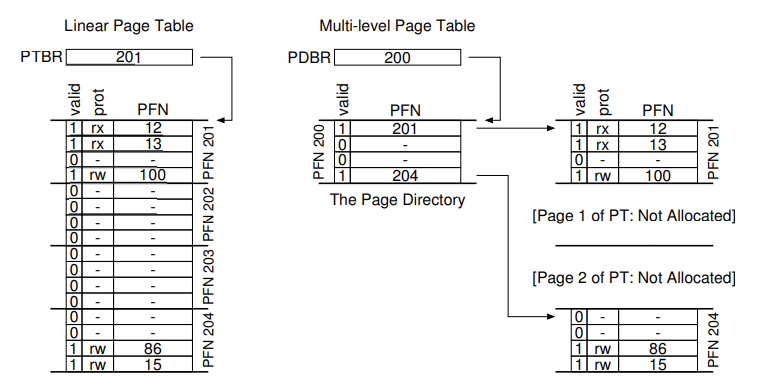
\includegraphics[width=0.65\textwidth]{src/multinivel.png}
    \caption{Paginación multinivel}
\end{figure}

A la izquierda está la clásica tabla de páginas lineal; aunque la mayoría de las regiones intermedias del espacio de direcciones no son válidas, aún se requiere espacio en la tabla de páginas asignado para esas regiones (es decir, las dos páginas intermedias de la tabla de páginas). A la derecha está una tabla de páginas multinivel. El directorio de páginas \textbf{marca solo dos páginas} de la tabla de páginas como \textbf{válidas} (la primera y la última); por lo tanto, solo esas dos páginas de la tabla de páginas residen en la memoria. Así se ve una forma de visualizar lo que está haciendo una tabla multinivel: simplemente hace que partes de la tabla de páginas lineal desaparezcan (liberando esos marcos para otros usos) y rastrea qué páginas de la tabla de páginas están asignadas mediante el directorio de páginas.

El directorio de páginas, en una tabla de dos niveles, contiene una entrada por cada página de la tabla de páginas. Consiste en un número de entradas del directorio de páginas (PDE). Un PDE (mínimamente) tiene un bit de validez y un número de marco de página (PFN), similar a un PTE. Sin embargo, como se mencionó antes, el significado de este bit de validez es ligeramente diferente: si el PDE es válido, significa que la page table que le sigue está presente o no, y si no es válido, significa que la page table no está presente.

Existe un registro llamado Page Directory Base Register (PDBR) que apunta a la dirección física del directorio de páginas.

\subsection{Ejemplo completo}
Supongamos que se tiene un pequeño espacio de direcciones de 16 KB, con páginas de 64 bytes. Así, tenemos un espacio de direcciones virtuales de 14 bits, con 8 bits para el VPN (número de página virtual) y 6 bits para el desplazamiento. Una tabla de páginas lineal tendría $2^8$ (256) entradas, incluso si solo se utiliza una pequeña porción del espacio de direcciones. Como se ve acontinuación:

\begin{figure}[h]
    \centering
    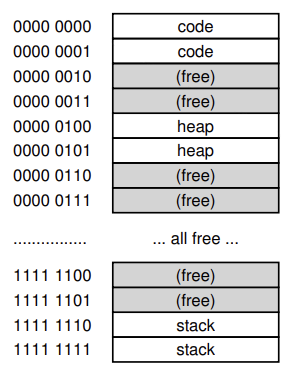
\includegraphics[width=0.3\textwidth]{src/lineal.png}
    \caption{Tabla de páginas lineal}
\end{figure}

En este ejemplo, las páginas virtuales 0 y 1 son para código, las páginas virtuales 4 y 5 para el montón (heap), y las páginas virtuales 254 y 255 para la pila; el resto de las páginas del espacio de direcciones no se utilizan.

Para construir una tabla de páginas de dos niveles para este espacio de direcciones, comenzamos con nuestra tabla de páginas lineal completa y la dividimos en unidades del tamaño de una página. Recuerda que nuestra tabla completa (en este ejemplo) tiene 256 entradas; supongamos que cada entrada de la tabla de páginas (PTE) tiene 4 bytes de tamaño. Por lo tanto, nuestra tabla de páginas ocupa 1 KB (256 × 4 bytes). Dado que tenemos páginas de 64 bytes, la tabla de páginas de 1 KB puede dividirse en 16 páginas de 64 bytes; cada página puede contener 16 entradas de la tabla de páginas.

Ahora necesitamos entender cómo tomar un VPN y usarlo primero para indexar en el directorio de páginas y luego en la página de la tabla de páginas. Recuerda que ambos son arrays de entradas; por lo tanto, solo necesitamos averiguar cómo construir el índice de cada uno a partir de partes del VPN. Primero indexemos en el directorio de páginas. Nuestra tabla de páginas en este ejemplo es pequeña: 256 entradas, distribuidas en 16 páginas. 

El directorio de páginas necesita una entrada por página de la tabla de páginas; por lo tanto, tiene 16 entradas. Como resultado, necesitamos cuatro bits del VPN para indexar en el directorio; usamos los cuatro bits superiores del VPN, de la siguiente manera:

\begin{figure}[h]
    \centering
    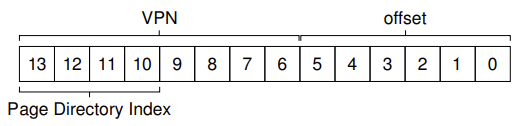
\includegraphics[width=0.5\textwidth]{src/direccionamiento.png}
    \caption{Direccionamiento}
\end{figure}

Una vez que extraemos el índice del directorio de páginas (PDIndex para abreviar) del VPN, podemos usarlo para encontrar la dirección de la entrada del directorio de páginas (PDE) con un cálculo simple:

\begin{equation*}
    \text{PDEAddr} = \text{PDBR} + (\text{PDIndex} \times \text{sizeof(PDE)})
\end{equation*}

Donde PDBR es el registro base del directorio de páginas, sizeof(PDE) es el tamaño de una entrada del directorio de páginas (en este caso, 4 bytes), y PDIndex es el índice del directorio de páginas que acabamos de calcular. 

Si la entrada del directorio de páginas está marcada como inválida, sabemos que el acceso es inválido y, por lo tanto, se lanza una excepción. Sin embargo, si el PDE es válido, tenemos más trabajo por hacer. Específicamente, ahora tenemos que obtener la entrada de la tabla de páginas (PTE) de la página de la tabla de páginas a la que apunta esta entrada del directorio de páginas. Para encontrar este PTE, debemos indexar en la parte de la tabla de páginas usando los bits restantes del VPN:

\begin{figure}[h]
    \centering
    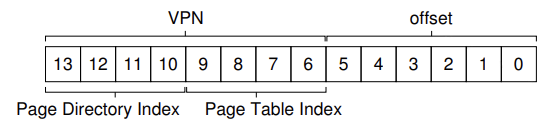
\includegraphics[width=0.6\textwidth]{src/pte2.png}
    \caption{Entrada de la tabla de páginas}
\end{figure}

Este índice de la tabla de páginas (PTIndex para abreviar) puede usarse para indexar en la tabla de páginas en sí, dándonos la dirección de nuestro PTE:
\begin{equation*}
    \text{PTEAddr} = (\text{PDE.PFN} \ll \text{SHIFT}) + (\text{PTIndex} \times \text{sizeof(PTE)})
\end{equation*}
Observa que el número de marco de página obtenido de la entrada del directorio de páginas debe desplazarse a la izquierda antes de combinarlo con el índice de la tabla de páginas para formar la dirección del PTE.

Ahora, llenaremos una tabla de páginas multinivel con algunos valores reales y traduciremos una dirección virtual.

\begin{figure}[h]
    \centering
    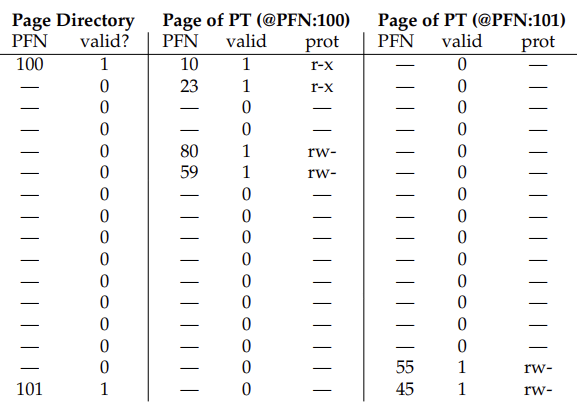
\includegraphics[width=0.47\textwidth]{src/pte3.png}
    \caption{Entrada de la tabla de páginas}
\end{figure}

En este ejemplo, tenemos dos regiones válidas en el page directory (al principio y al final), y un número de mapeos inválidos en el medio. En la página física 100, tenemos la primera página de 16 entradas de la tabla de páginas para los primeros 16 VPN en el espacio de direcciones.

Esta página de la tabla de páginas contiene los mapeos para los primeros 16 VPN; en nuestro ejemplo, los VPN 0 y 1 son válidos (el segmento de código), al igual que los 4 y 5 (el montón). Por lo tanto, la tabla tiene información de mapeo para cada una de esas páginas. El resto de las entradas están marcadas como inválidas.

La otra página válida de la tabla de páginas se encuentra en el marco de página 101. Esta página contiene los mapeos para los últimos 16 VPN del espacio de direcciones.

En el ejemplo, los VPN 254 y 255 (la pila) tienen mapeos válidos. Se ve que el espacio se puede ahorrar con una estructura indexada multinivel. En este ejemplo, en lugar de asignar las dieciséis páginas completas para una tabla de páginas lineal, asignamos solo tres: una para el directorio de páginas, y dos para los fragmentos de la tabla de páginas que tienen mapeos válidos. Los ahorros para espacios de direcciones grandes (de 32 o 64 bits) podrían ser obviamente mucho mayores.

\subsection{Ventajas y desventajas}
Ventajas:
\begin{itemize}
    \item Se almacena lo que se mapea, no se desperdicia espacio.
    \item El tamaño total del page directory mas las page tables es lineal respecto a la memoria ocupada.
\end{itemize}
Desventajas:
\begin{itemize}
    \item Cada vez que se necesita traducir de virtual a físico, se requiere acceder a dos tablas.
\end{itemize}

\newpage
\subsection{Método de resolución de ejercicios de paginación}
\subsubsection{Paginación Lineal}

\begin{figure}[h]
    \centering
    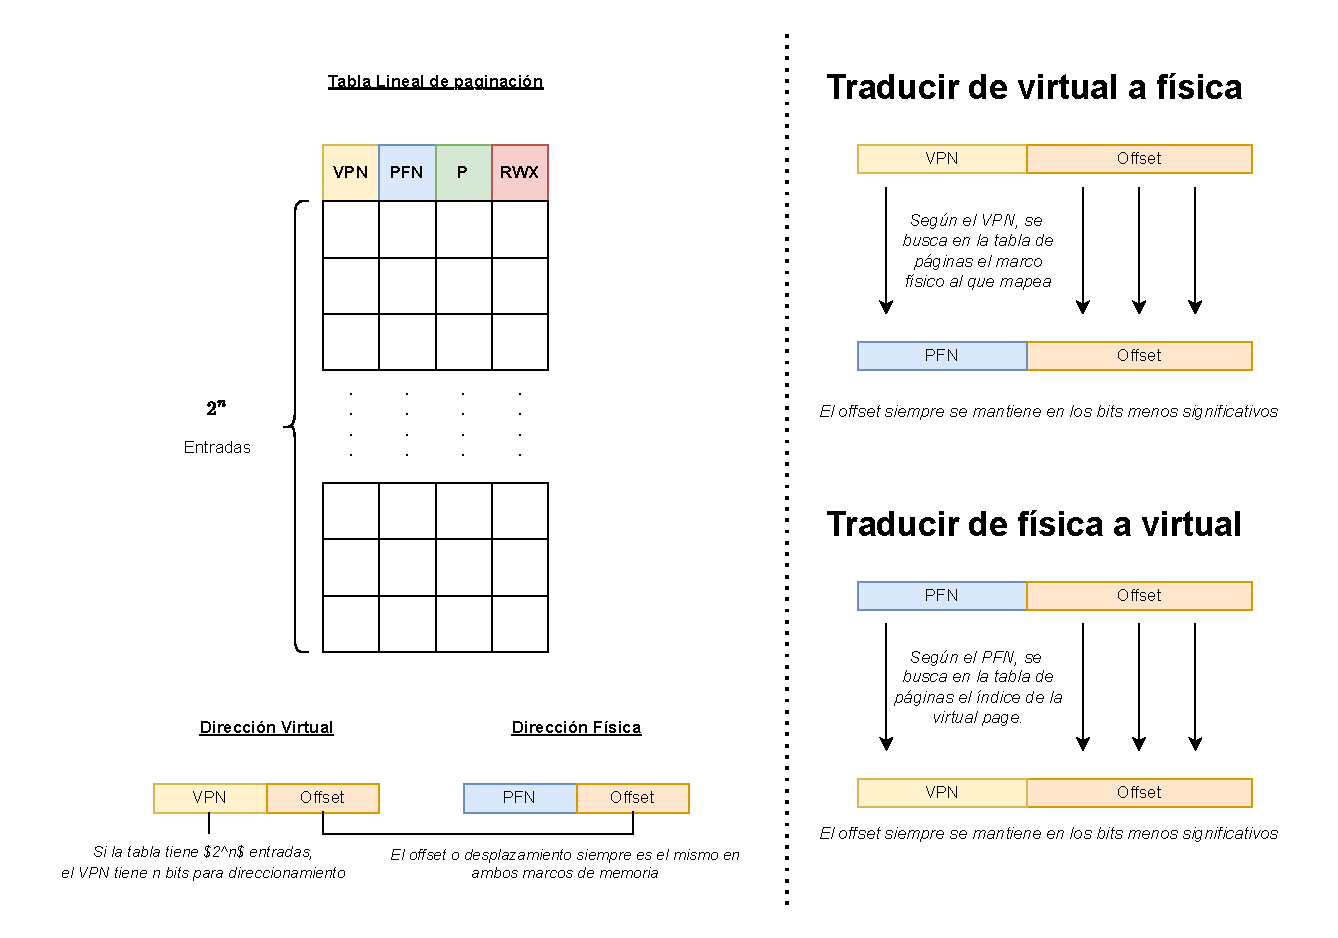
\includegraphics[width=0.95\textwidth]{src/paglineal.pdf}
    \caption{Paginación lineal}
\end{figure}

En el paso de traducción hay que tener en cuenta posibles casos no tan comunes:
\begin{itemize}
    \item El mapeo de virtual a físico no es necesariamente inyectivo, es decir, una dirección física puede ser mapeada a varias direcciones virtuales.
    \item Una consecuencia de ese mapeo no inyectivo es que si hay que traducir una dirección física a una virtual, no se puede hacer de forma única.
    \item Se produce un \textbf{page fault} cuando se intenta acceder a una dirección virtual que no está mapeada a una dirección física.
    \item Si se habla de legalidad de manejo de una dirección, hay que tener en cuenta los bits de protección de la PTE.
    \item Cuando el bit de presencia es 0, se produce un page fault.
\end{itemize}
\newpage
\subsubsection{Paginación Multinivel}
Hay una convención que se sigue para representar la distribución de bits en una dirección virtual. En el caso de la paginación multinivel, se divide la dirección virtual en tres partes:

\begin{figure}[h]
    \centering
    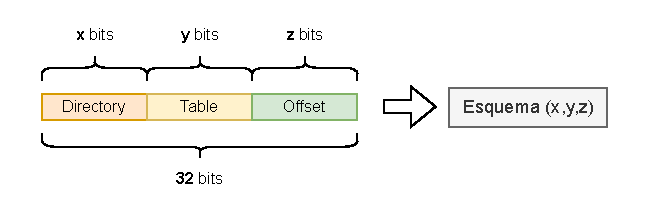
\includegraphics[width=0.85\textwidth]{src/convencion.pdf}
    \caption{Paginación multinivel - Convención}
\end{figure}

A grandes rasgos, la dirección virtual se divide en tres partes cuyas funciones son:
\begin{enumerate}
    \item \textbf{PDIndex}: Se usa para indexar en el directorio de páginas, que contiene las direcciones de las tablas de páginas. El registro base de esta estructura es el CR3.
    \item \textbf{PTIndex}: Se usa para indexar en la tabla de páginas, que contiene las direcciones físicas de las páginas.
    \item \textbf{Offset}: Se usa para indexar en la página física.
\end{enumerate}

Cuando los ejercicios mencionan i386, se refieren a la arquitectura de 32 bits de Intel. Aquí se tiene un esquema (10,10,12):

\begin{figure}[h]
    \centering
    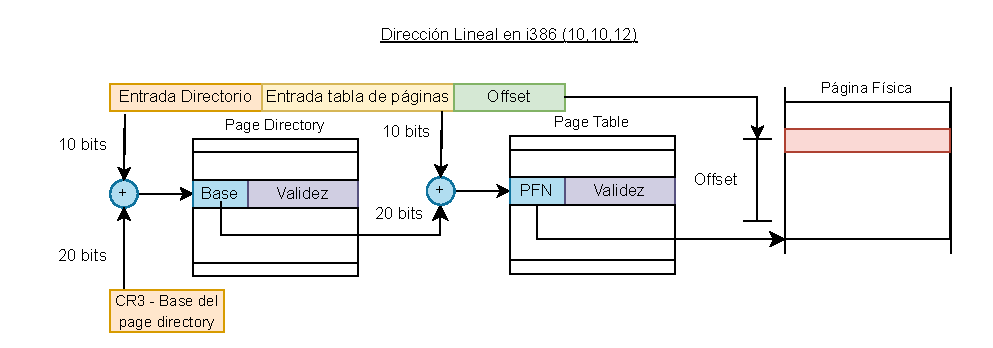
\includegraphics[width=0.95\textwidth]{src/i386.pdf}
    \caption{Paginación multinivel - i386}
\end{figure}

\textbf{Método de traducción}:
\begin{enumerate}
    \item Se extraen los bits de PDIndex y se indexa en el directorio de páginas.
    \item Una vez se tenga la dirección de la tabla de páginas, se extraen los bits de PTIndex y se indexa en la tabla de páginas.
    \item Se extraen los bits de offset y se indexa en la página física.
\end{enumerate}

\newpage
\section{Ejercicios de Examen}
\subsection{Ejercicio 1 - Parcial 1 2022}
El siguiente código de máquina y su desensamblado RISC-V \textbf{computa la suma prefijo en el mismo arreglo} (in-place prefix sum). El arreglo $a$ está en el segmento ELF .bss y empieza en 0x2FC0 y termina en 0x3008 \textbf{exclusive}. Como sus elementos son \texttt{unsigned long}, cada uno ocupa 8bytes y por lo tanto tiene 9 elementos.

\begin{verbatim}
0000000000000634 <main>:
634: 0613                                li         a2,0x3008         # <__BSS_END__> &a[9]
636: b206                                li         a5,0x2FC8         # <a+0x8> &a[1]
638: 6398                                ld         a4,0(a5)          # a4 = a[i]
63a: fff87b683                           ld         a3,-8(a5)         # a3 = a[i-1]
63e: 9736                                add        a4,a4,a3          # a4 = a[i] + a[i-1]
640: e398                                sd         a4,0(a5)          # a[i] = a4
642: 07a1                                addi       a5,a5,8           # i++
644: fec79ae3                            bne        a5,a2,0x638       # <main+0x10>, "i < 9"
648: 8082                                ret
\end{verbatim}

Escribir la \textbf{traza de memoria} completa que genera la ejecución del proceso \textbf{incluyendo los instruction fetch}.

\begin{itemize}
    \item Inicialización: Instruction fetch de la dirección 0x634.
    \item Inicialización: Instruction fetch de la dirección 0x636.
    \item Vuelta 1: 0x638, 0x2FC8, 0x63A, 0x2FC0, 0x63e, 0x640, 0x2FC8, 0x642, 0x644
    \item Vuelta 2: 0x638, 0x2FD0, 0x63A, 0x2FC8, 0x63e, 0x640, 0x2FD0, 0x642, 0x644
    \item Vuelta 3: 0x638, 0x2FD8, 0x63A, 0x2FD0, 0x63e, 0x640, 0x2FD8, 0x642, 0x644
    \item Vuelta 4: 0x638, 0x2FE0, 0x63A, 0x2FD8, 0x63e, 0x640, 0x2FE0, 0x642, 0x644
    \item Vuelta 5: 0x638, 0x2FE8, 0x63A, 0x2FE0, 0x63e, 0x640, 0x2FE8, 0x642, 0x644
    \item Vuelta 6: 0x638, 0x2FF0, 0x63A, 0x2FE8, 0x63e, 0x640, 0x2FF0, 0x642, 0x644
    \item Vuelta 7: 0x638, 0x3000, 0x63A, 0x2FF8, 0x63e, 0x640, 0x3000, 0x642, 0x644
    \item Fin: Instruction fetch de la dirección 0x648.
\end{itemize}

\subsection{Ejercicio 2 - Parcial 1 2022}
Supongamos que en trampoline.S la rutina en ensamblador RISC-V que guarda los registros de espacio de usuario se comete un pequeño error por culpa del gato

\newpage
\subsection{Ejercicio 4 - Parcial 1 2022}
Tenemos un esquema de paginación de RISC-V con páginas de 4KiB de 3 niveles con formato 9,9,9,12 $->$ 44,12 como muestra la siguiente figura:

\begin{figure}[h]
    \centering
    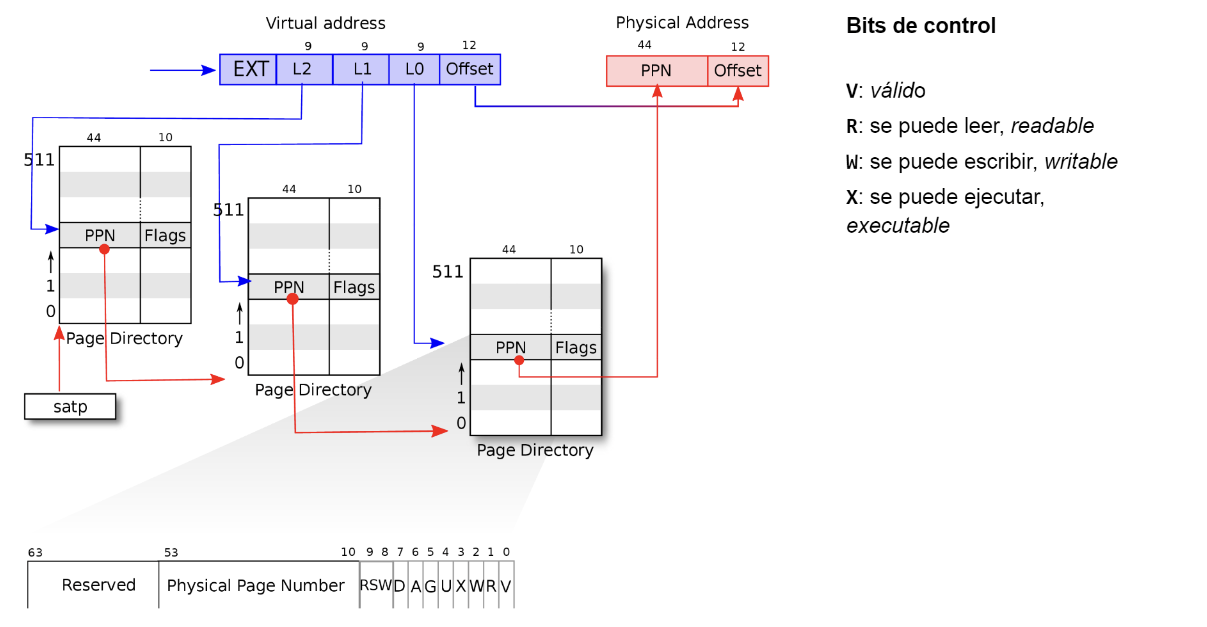
\includegraphics[width=0.95\textwidth]{src/ej4.png}
    \caption{Esquema de paginación- Ejercicio de Parcial}
\end{figure}

Supongamos que tenemos el registro de paginación apuntando al marco físico satp=0x00000000FE0

\begin{figure}[h]
    \centering
    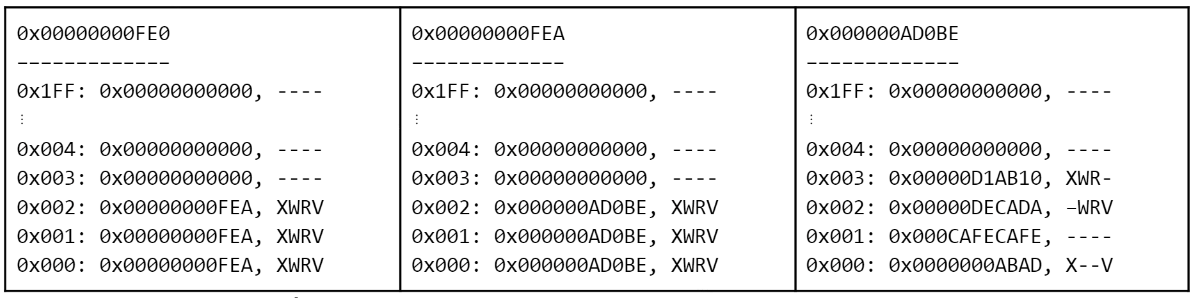
\includegraphics[width=0.95\textwidth]{src/ej4.1.png}
    \caption{Registro de paginación - Ejercicio de Parcial}
\end{figure}

\begin{enumerate}
    \item Traducir de \textbf{virtual a física} las direcciones:
    \begin{enumerate}
        \item 0x0000,
        \item 0x1000.
    \end{enumerate}
    \item Traducir de la dirección física 0xDECADA980 a \textbf{todas} las virtuales que la apuntan.
\end{enumerate}

Por lo pronto tenemos una paginación de 3 niveles con esquema 9,9,9,12. Esto quiere decir que los primeros 9 bits me indexan el primer directorio de páginas, los siguientes 9 bits me indexan el segundo directorio de páginas, los siguientes 9 bits me indexan la tabla de páginas y los últimos 12 bits me indexan la página física.
\textbf{Punto 1:}

0x0000: 000 0000 00 $|$ 00 0000 000 $|$ 0 0000 0000 $|$ 0000 0000 0000
\begin{itemize}
    \item Índice 0 en el primer directorio de páginas.
    \item Índice 0 en el segundo directorio de páginas.
    \item Índice 0 en la tabla de páginas.
    \item Mapea a la dirección 0x0000000ABAD000. Con un offset de 0x000.
\end{itemize}
0x1000: 000 0000 00 $|$ 00 0000 000 $|$ 0 0000 0001 $|$ 0000 0000 0000
\begin{itemize}
    \item Índice 0 en el primer directorio de páginas.
    \item Índice 0 en el segundo directorio de páginas.
    \item Índice 1 en la tabla de páginas.
    \item No mapea ya que la entrada no está presente.
\end{itemize}
\textbf{Punto 2:}
Hay varias direcciones de memoria virtual que apuntan a la dirección física 0xDECADA980. Para encontrarlas, se debe recorrer la tabla de páginas y los directorios de páginas. Van a haber varios caminos que vayan a parar al mismo lugar, lo único que se mantiene fijo es el offset 980.

\subsection{Ejercicio 5 - Parcial 1 2022}
A la luz del esquema de paginación del ejercicio 4, indicar de que manera esquemática que es lo que pasaría con la traza de memoria respecto a la ejecución de un proceso corriendo el código máquina del ejercicio 1.

A modo de ilustración, si se tiene por ejemplo la dirección de instructión fech en 0x634, se tiene:

000 0000 00 $|$ 00 0000 000 $|$ 0 0000 0000 $|$ 0110 0011 0100 
\begin{itemize}
    \item Índice 0 en el primer directorio de páginas.
    \item Índice 0 en el segundo directorio de páginas.
    \item Índice 0 en la tabla de páginas.
    \item Mapea a la dirección 0x0000000ABAD634. Con un offset de 0x634.
\end{itemize}

Esto quiere decir que el acceso mediante la instrucción fetch a la dirección 0x634 se traduce a la dirección física \textbf{0x0000000ABAD634}.
\newpage
\subsection{Ejercicio Parcial 2021}

\begin{figure}[h]
    \centering
    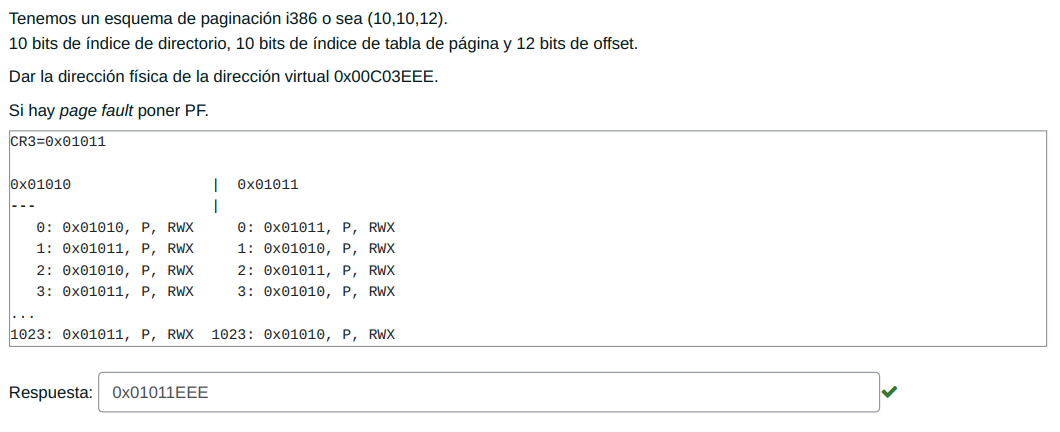
\includegraphics[width=0.95\textwidth]{src/ejercicio2021.png}
    \caption{Ejercicio Parcial 2021}
\end{figure}

\begin{figure}[h]
    \centering
    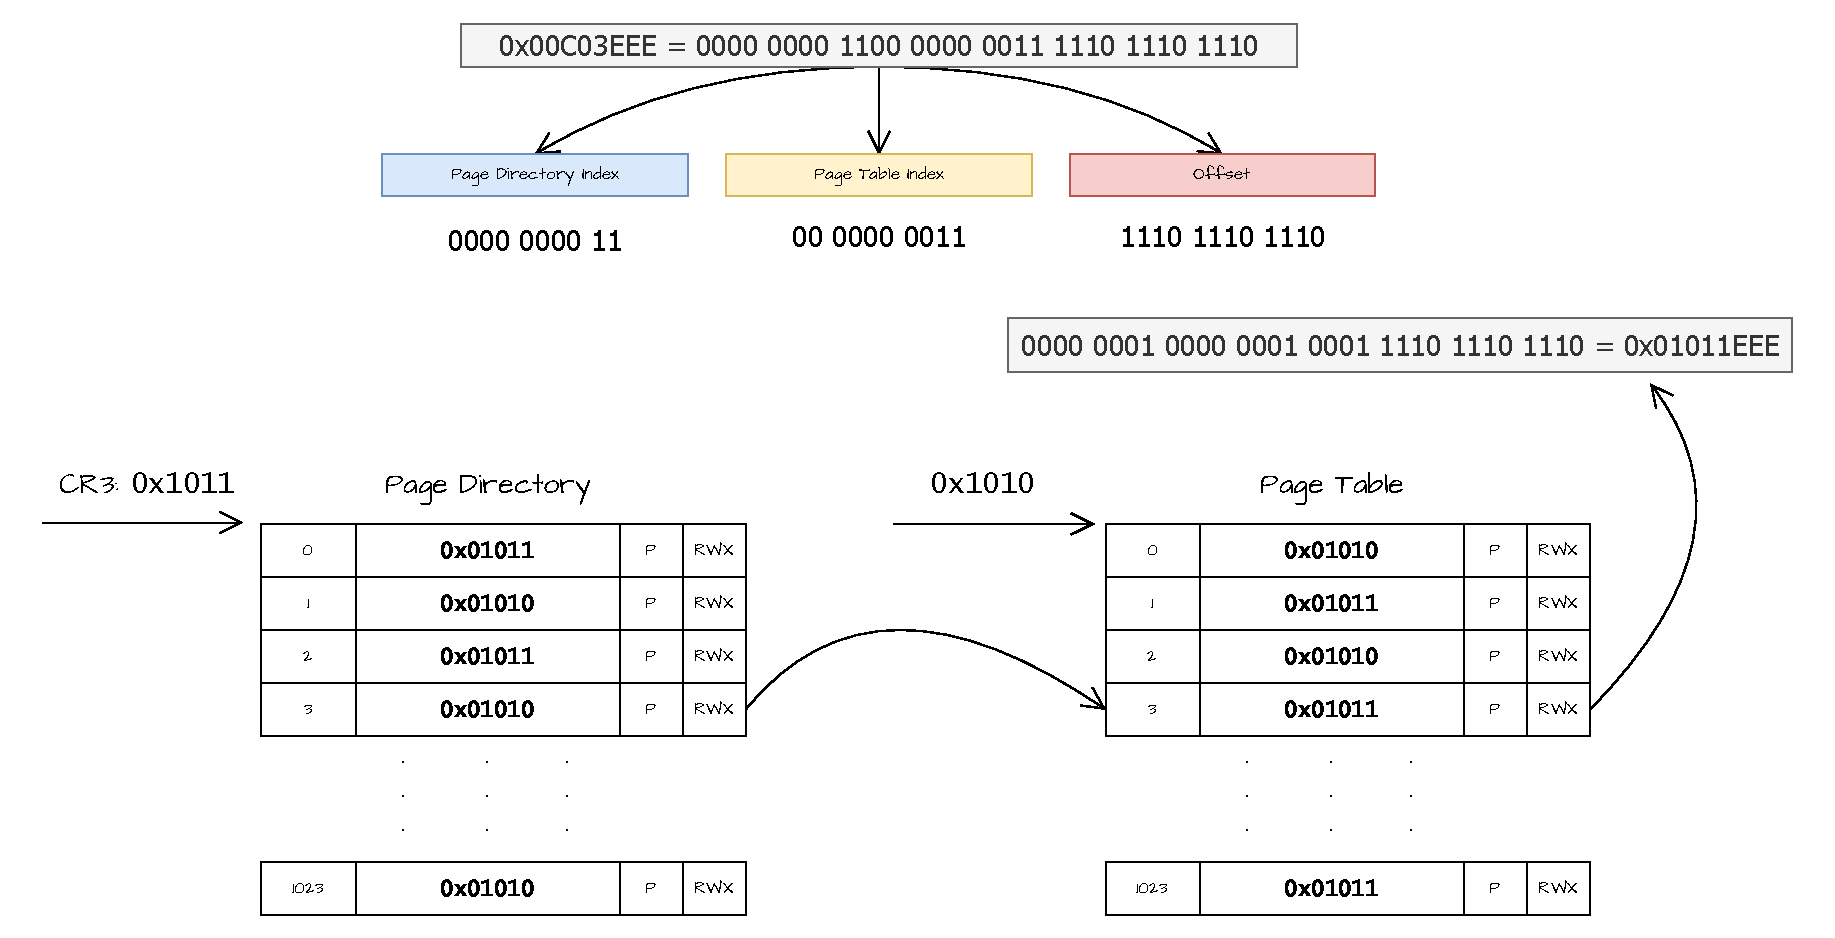
\includegraphics[width=0.95\textwidth]{src/2021.pdf}
    \caption{Ejercicio Parcial 2021 - Solución}
\end{figure}

\end{document}
